

\documentclass[preprint,12pt]{elsarticle}
\usepackage{caption} 
\usepackage{color}%临时添加,
\usepackage{amssymb,hyperref,booktabs,multirow,multicol,ifthen}
\usepackage{enumerate}
\usepackage{nomencl}
\usepackage{float}
\usepackage{graphics}
\usepackage{framed}


\renewcommand{\nomgroup}[1]
{%Mathematical symbols
\ifthenelse{\equal{#1}{G}}{\item[\textbf{Greek letters}]}{%
\ifthenelse{\equal{#1}{S}}{\item[\textbf{Subscripts}]}{%
\ifthenelse{\equal{#1}{U}}{\item[\textbf{Superscripts}]}{
\ifthenelse{\equal{#1}{C}}{\item[\textbf{Constants}]}{
\ifthenelse{\equal{#1}{M}}{\item[\textbf{Mathematical symbols}]}{
}%几个类别需要几个括号
}
}
}
}%几个类别需要几个括号
}%对应1]
\makenomenclature

 \usepackage{amsmath}%

 \usepackage{lineno}%

\usepackage{bm}%

\captionsetup[figure]{font=small,labelfont=bf,labelsep=period}%

\renewcommand{\figurename}{Fig.}%

\journal{Applied Energy}

\begin{document}

\begin{frontmatter}



\title{A novel 1000\,MW double-reheat ultra supercritical system with turbine-extraction-heated air preheaters and low-temperature economizers}


\author[hust,ncst]{Lei Zhang}
\ead{zhanglei@ncst.edu.cn}	
\author[hust]{Jiayi Zhao}
\author[hust]{Tao Yang\corref{cor1}} %I am not sure how to delete the extra comma after Yang's name--there is a comma after the "a" superscript that needs to be removed.
\ead{hust\_yt@hust.edu.cn}	
\author[hust]{Yanping Zhang}
\author[hust]{Wei Gao}


\address[hust]{School of Energy and Power Engineering, Huazhong University of Science and Technology, Wuhan 430074, China}
\address[ncst]{College of Metallurgy and Energy, North China University of Science and Technology, Tangshan 063009, China}
\cortext[cor1]{Corresponding author}

\begin{abstract}%修改到300字以内
The double-reheat ultra-supercritical (USC) unit has received significant attention because of its high efficiency and energy-saving effects.
The optimal design of the unit's thermal system is still under consideration, however.
In this paper, an optimized system for reasonable fluid heat transfer temperature-matching and higher efficiency is proposed.
This novel system uses turbine extractions as heat sources for air preheaters and low-pressure economizers to absorb economizer outlet flue gas heat, thereby realizing the joint optimization of the air preheat process and the regenerative system.
Models were built to compare the energetic performance of the novel system and that of the reference system.
In addition, thermodynamic analyses under partial load operation conditions were conducted. 
Exergy analysis was used to identify the exergy destruction changes of the transformed parts and to analyze the cause of the changes.
The results show that the novel system largely decreased the exergy destruction rate of the air preheat process and improved the system's thermal performance.
Furthermore, the novel system increased the temperature of secondary air and reduced the overall superheat degree of several extractions.
Theoretically, with an overall exergy efficiency of 48.73\%, the novel system can reduce SCE
%I don't think the "SCE" acronym has been introduced yet. Write it out in full here? 
consumption by nearly 5.5\,g/kWh under the THA load
%Same for THA---write out in full?
if the temperature of the flue gas entering the electrostatic precipitator is set to 95$^\circ$C.
Moreover, the novel system has advantages for coal-saving under the partial load condition.
Ultimately, the results indicate that the novel system can improve the performance of the double-reheat USC unit and may provide a theoretical basis for its optimization.

\end{abstract}

\begin{keyword}
Double-reheat \sep ultra-supercritical power plant \sep exergy analysis \sep air preheat process \sep thermodynamic analysis
\end{keyword}

\end{frontmatter}

\begin{multicols}{2}
\printnomenclature[1.5cm]{}
\end{multicols}



\section{Introduction}
\label{sec1:intro}
Coal is still the main fossil fuel resource for the production of electricity globally, according to~\cite{Ouedraogo2013Energy}. 
In China, coal–fired power generation accounts for more than 70\% of the total electricity generation and subsequently contributes almost 50\%, 37\%, 33\%, and 55\% to the SO$_X$, NO$_X$, dust, and CO$_X$ emission volumes, respectively~\cite{Zhang2010Analysis}.
Statistics show that China has been the largest producer and consumer of energy worldwide since 2013~\cite{Petroleum2014BP}. 
In 2016, Chinese coal production fell by 7.9\% and the price of steam coal increased by over 60\%~\cite{Petroleum2017BP}. 
Improving system efficiency and reducing coal consumption remain the primary tasks to be considered in power plant design. Nowadays ultra-supercritical (USC) power plants with large capacities and high parameters are considered to be feasible ways to save energy; as such, their usage has spread rapidly worldwide.
The double-reheat USC unit is a new generation of USC unit that can improve thermal performance when compared with a single reheat unit~\cite{Zhao2017Exergy}. 
According to~\cite{Zhao2017Exergy}, a double reheat unit with the inlet parameter 30.0\,MPa/600/620/620$^\circ$C improves the heat efficiency by 2.4\%-2.6\% when compared with a commonly used USC unit with the inlet parameter 25.0\,MPa/600/600$^\circ$C.
 The United States built the first double-reheat unit with the main parameter 34.4 MPa/649/566/566$^\circ$C in the 1960s.
 Two 700 MW double-reheat USC units were put into operation in Japan in 1990. 
 The process of building five double-reheat USC units began in China in 2012, and three of these units were put into operation in 2015.
 Over the past few decades, double-reheat USC units have received increasing attention due to their rapid development worldwide.

  

Though the high live steam pressure and temperature of the USC unit improve its efficiency, there are still some imperfections that limit the improvement of the unit's performance. 
In order to perform an in-depth analysis of the system, Zhao Z et al.~\cite{Zhao2017Exergy} studied the exergy distribution system for a 1000\,MW double-reheat USC power plant and determined the main causes of exergy destruction on the steam turbine.
Rashidi et al.~\cite{Rashidi2014Thermodynamic} performed a thermodynamic analysis of a double-reheat steam power plant.
According to Ref.~\cite{Wu2014Component}, component- and process-based exergy evaluations were performed on a coal-fired power plant in China, thereby helping researchers to identify energy-saving strategies.
It was pointed out that the exergy destruction in the heat transfer process accounts for the largest proportion.
%largest proportion of what? Of exergy destruction overall?

Compared with the common USC system, the double-reheat system has some typical problems, such as the double-reheat ratio that is chosen and the high superheat degree of the first several extractions.
Other common problems include the high boiler exhaust temperature, which leads to unreasonable energy-level matching and significant exergy destruction. 

To identify reasonable reheat parameters, Zhou et al.~\cite{Zhou2016Parametric} carried out a parametric analysis and system optimization of double-reheat ultra-supercritical power plants based on exergy analysis and economic analysis. The results showed that reasonable reheat parameters and reheat stage numbers can improve the double-reheat system's performance.


To reduce the superheat degree of the extractions, Xu et al.~\cite{Xu2015Optimum} investigated the thermal performance of the steam and water cycle with a single reheat after the installation of an additional outer steam cooler (AOC).
The results showed that the AOC is an effective method of reducing the superheat degree and improving the efficiency of the unit.
Li et al.~\cite{Li2014Thermodynamic} proposed a system that uses ten-stage extractions and two outer steam coolers. 
The results of the thermodynamic and techno-economic analyses showed that this system can lower the cost of electricity to 55.89 USD/MWh.
In addition, Kjaer~\cite{Kjaer2010A} proposed a regenerative steam turbine for utilizing the superheat degree of the extractions.
In this design, part of the extraction from the high pressure turbine enters the additional regenerative steam turbine rather than the regenerative heater.
Extractions from the intermediate pressure turbine are replaced by those from the regenerative steam turbine.
The superheat degree of the extraction is significantly reduced in this design and the exergy destruction of regenerative heaters is likewise reduced, thereby resulting in an overall improvement in efficiency.

To reuse the energy of the exhaust flue gas, Xu et al.~\cite{Xu2013Techno} proposed a low-pressure economizer (LPE) based on data compiled from some typical 1000\,MW power generation units in China. Four possible arrangements for LPE installation were proposed and their energy-saving effects were compared.
The results indicated that the LPE connected with the higher-temperature section of the condensate line created a greater reduction in the standard coal equivalent (SCE). %"greatest"? 
Wang et al.~\cite{Wang2012Application} investigated energy- and water-saving measures and the reduction of CO$_2$ after the installation of an LPE.
The results showed that the optimized measures can reduce SCE by 2-4\,g/kWh.
Stevanovic et al.~\cite{Stevanovic2014Efficiency} proposed an additional high-pressure economizer installed at a long-term running lignite-fired power plant.
The results showed that more than 30\,MW of the flue gas waste heat was recovered, creating an improvement in gross efficiency of 0.53\% and 9.4\,MW extra output power.
Xu et al.~\cite{Xu2013A} divided the air preheater into two stages to reduce the temperature difference in the heat transfer process.
%"divided the air preheater process"? Or was the preheater itself actually divided?
A LPE was also installed between the two air preheaters to obtain an appropriate flue gas temperature range.
Thermodynamic and technic-economic analyses were conducted to reveal the performance improvement.
It was found that the SCE consumption was reduced by 6.7\,g/kWh. %"techno-economic" is used earlier in the paper. Which expression is correct?

The installation of an LPE has some other benefits, such as improvements in electrostatic precipitator collection efficiency~\cite{Li2016Low}.

Given that boiler design and thermal system design belong to different research areas, boiler design is studied as a whole apart from the joint optimization of the boiler heat transfer process and regenerative process.

In this paper, a novel system based on a 1000\,MW double-reheat USC reference system is proposed to realize boiler and regenerative system energy cascade utilization. 
The novel system realized the reasonable temperature-matching of flue gas, air, extraction steam, and condensate water by using turbine-extraction-heating air preheaters (EAPHs) and LPEs.
Specifically, this study included the following tasks: (1) modeling the novel system and reference system with EBSILON® Professional; (2) using exergy analysis to compare both systems' exergy efficiency, exergy destruction distribution, and subsystem performance change; and (3) analyzing both systems' thermal performances under off-design conditions.



\section{Optimization of the double-reheat USC system}
\label{sec2:system intro}
\subsection{Reference system in operation} % (fold)
\label{sub2:ref intro}
A typical coal-fired double-reheat USC power plant in operation was chosen as the reference unit.
The parameter settings at maximum continuous power were 310\,bar/600$^\circ$C for the main steam, 610$^\circ$C for the reheat steam pressure, 33.5\% for the proportion of single-reheat steam pressure to main steam pressure, and 33\% for the proportion of double-reheat steam pressure to single-reheat steam pressure~\cite{Zhao2017Exergy}.
The output power of the reference system under the design condition was 1000 MW.
The unit consisted of one super-high pressure cylinder (VHP), one high-pressure cylinder (HP), one intermediate-pressure cylinder (IP), and two low-pressure cylinders (LPs).
A regenerative system with four high-pressure regenerative heaters (HRHs), five low-pressure regenerative heaters (LRHs), and one deaerator (DEA) was adopted.
In addition, two additional outer steam coolers (AOC1, AOC2) were used to cool two extractions due to their high super-heat degree. The exhaust steam pressure of the steam turbine was set to 4.5\,kPa. Its simplified schematic is presented in Fig.~\ref{fig:reference_system}.

\begin{figure}[htbp]
\centering
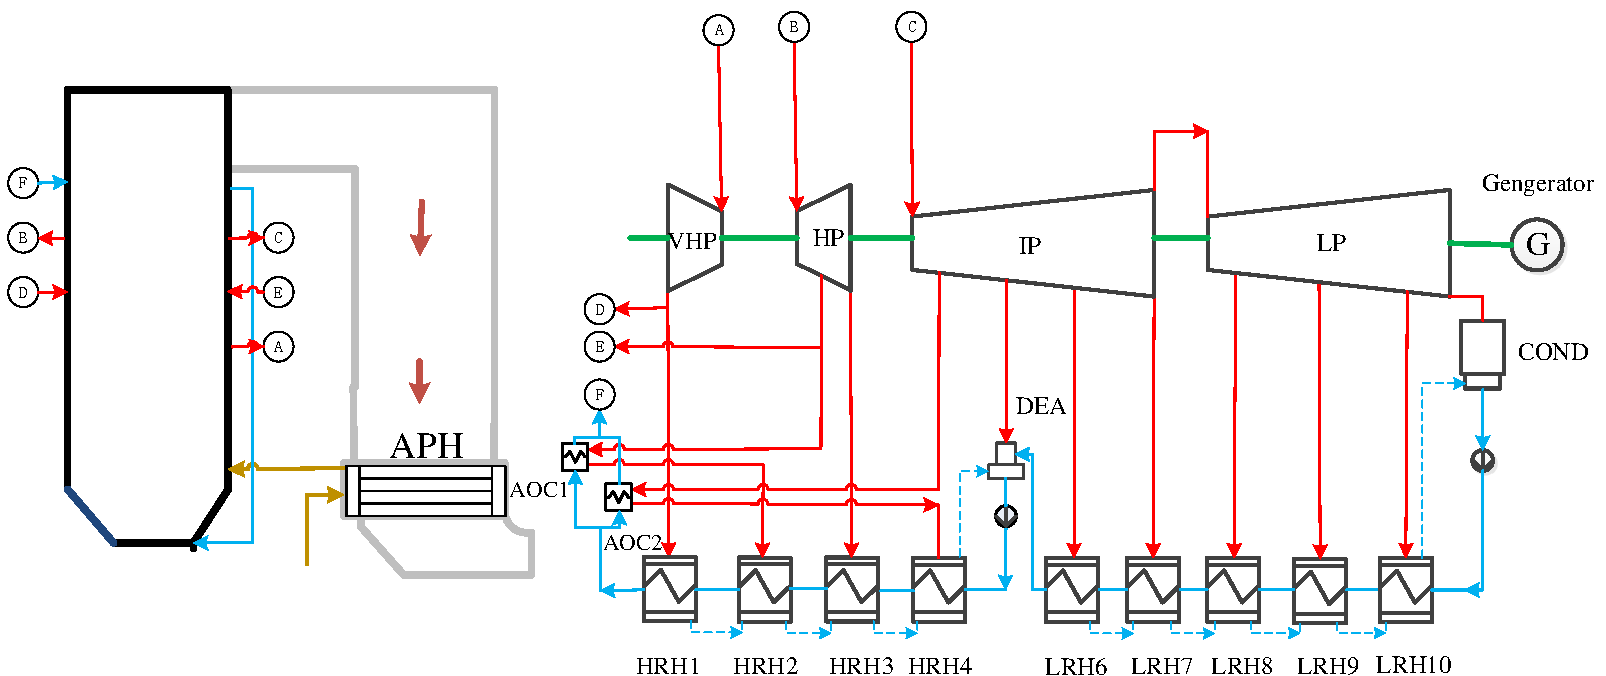
\includegraphics[width=1\textwidth]{fig/reference_system}
\caption{Schematic of the reference system} 
\label{fig:reference_system}
\end{figure}
%从参考系统的锅炉虽然仍然采用Π型布置,但其内部受热面和传统一次再热锅炉有较大区别。
The system's boiler heat transfer surface arrangement is shown in Fig.~\ref{fig:boiler_surface}. 
The boiler furnace is composed of the membrane wall; along the flue gas flow direction lie the low-temperature superheater (Lts) screen tube, the cold segment of the first high-temperature reheater (Csf), the cold segment of the second high-temperature reheater (Css), the high-temperature super-heater (Hts), the hot segment of the first high-temperature reheater (Hsf), and the hot segment of the second high-temperature reheater (Hss).
After Hsf and Hss, the flue gas channel is divided into the front-duct flue and the back-duct flue.
The front duct arranges the first low-temperature reheater (Ltfr) and the front-duct economizer (Feco).
The back duct arranges the second low-temperature reheater (Ltsr) and the back-duct economizer (Beco).
The air preheater (APH) is arranged in the vertical shaft. %What does "arranges" mean in these sentences? 

From the arrangement of the heating transfer surfaces, the boiler can be divided into two parts: the part performing the heat absorption for the water/steam process in the furnace and the APH that completes the air preheat process.
It can be seen that most heating surfaces of the boiler are arranged in the furnace, while the horizontal flue and vertical shaft are only equipped with APH.
This means that the horizontal flue and vertical shaft leave sufficient space for the installation of other equipment.

\begin{figure}[htbp]
\centering
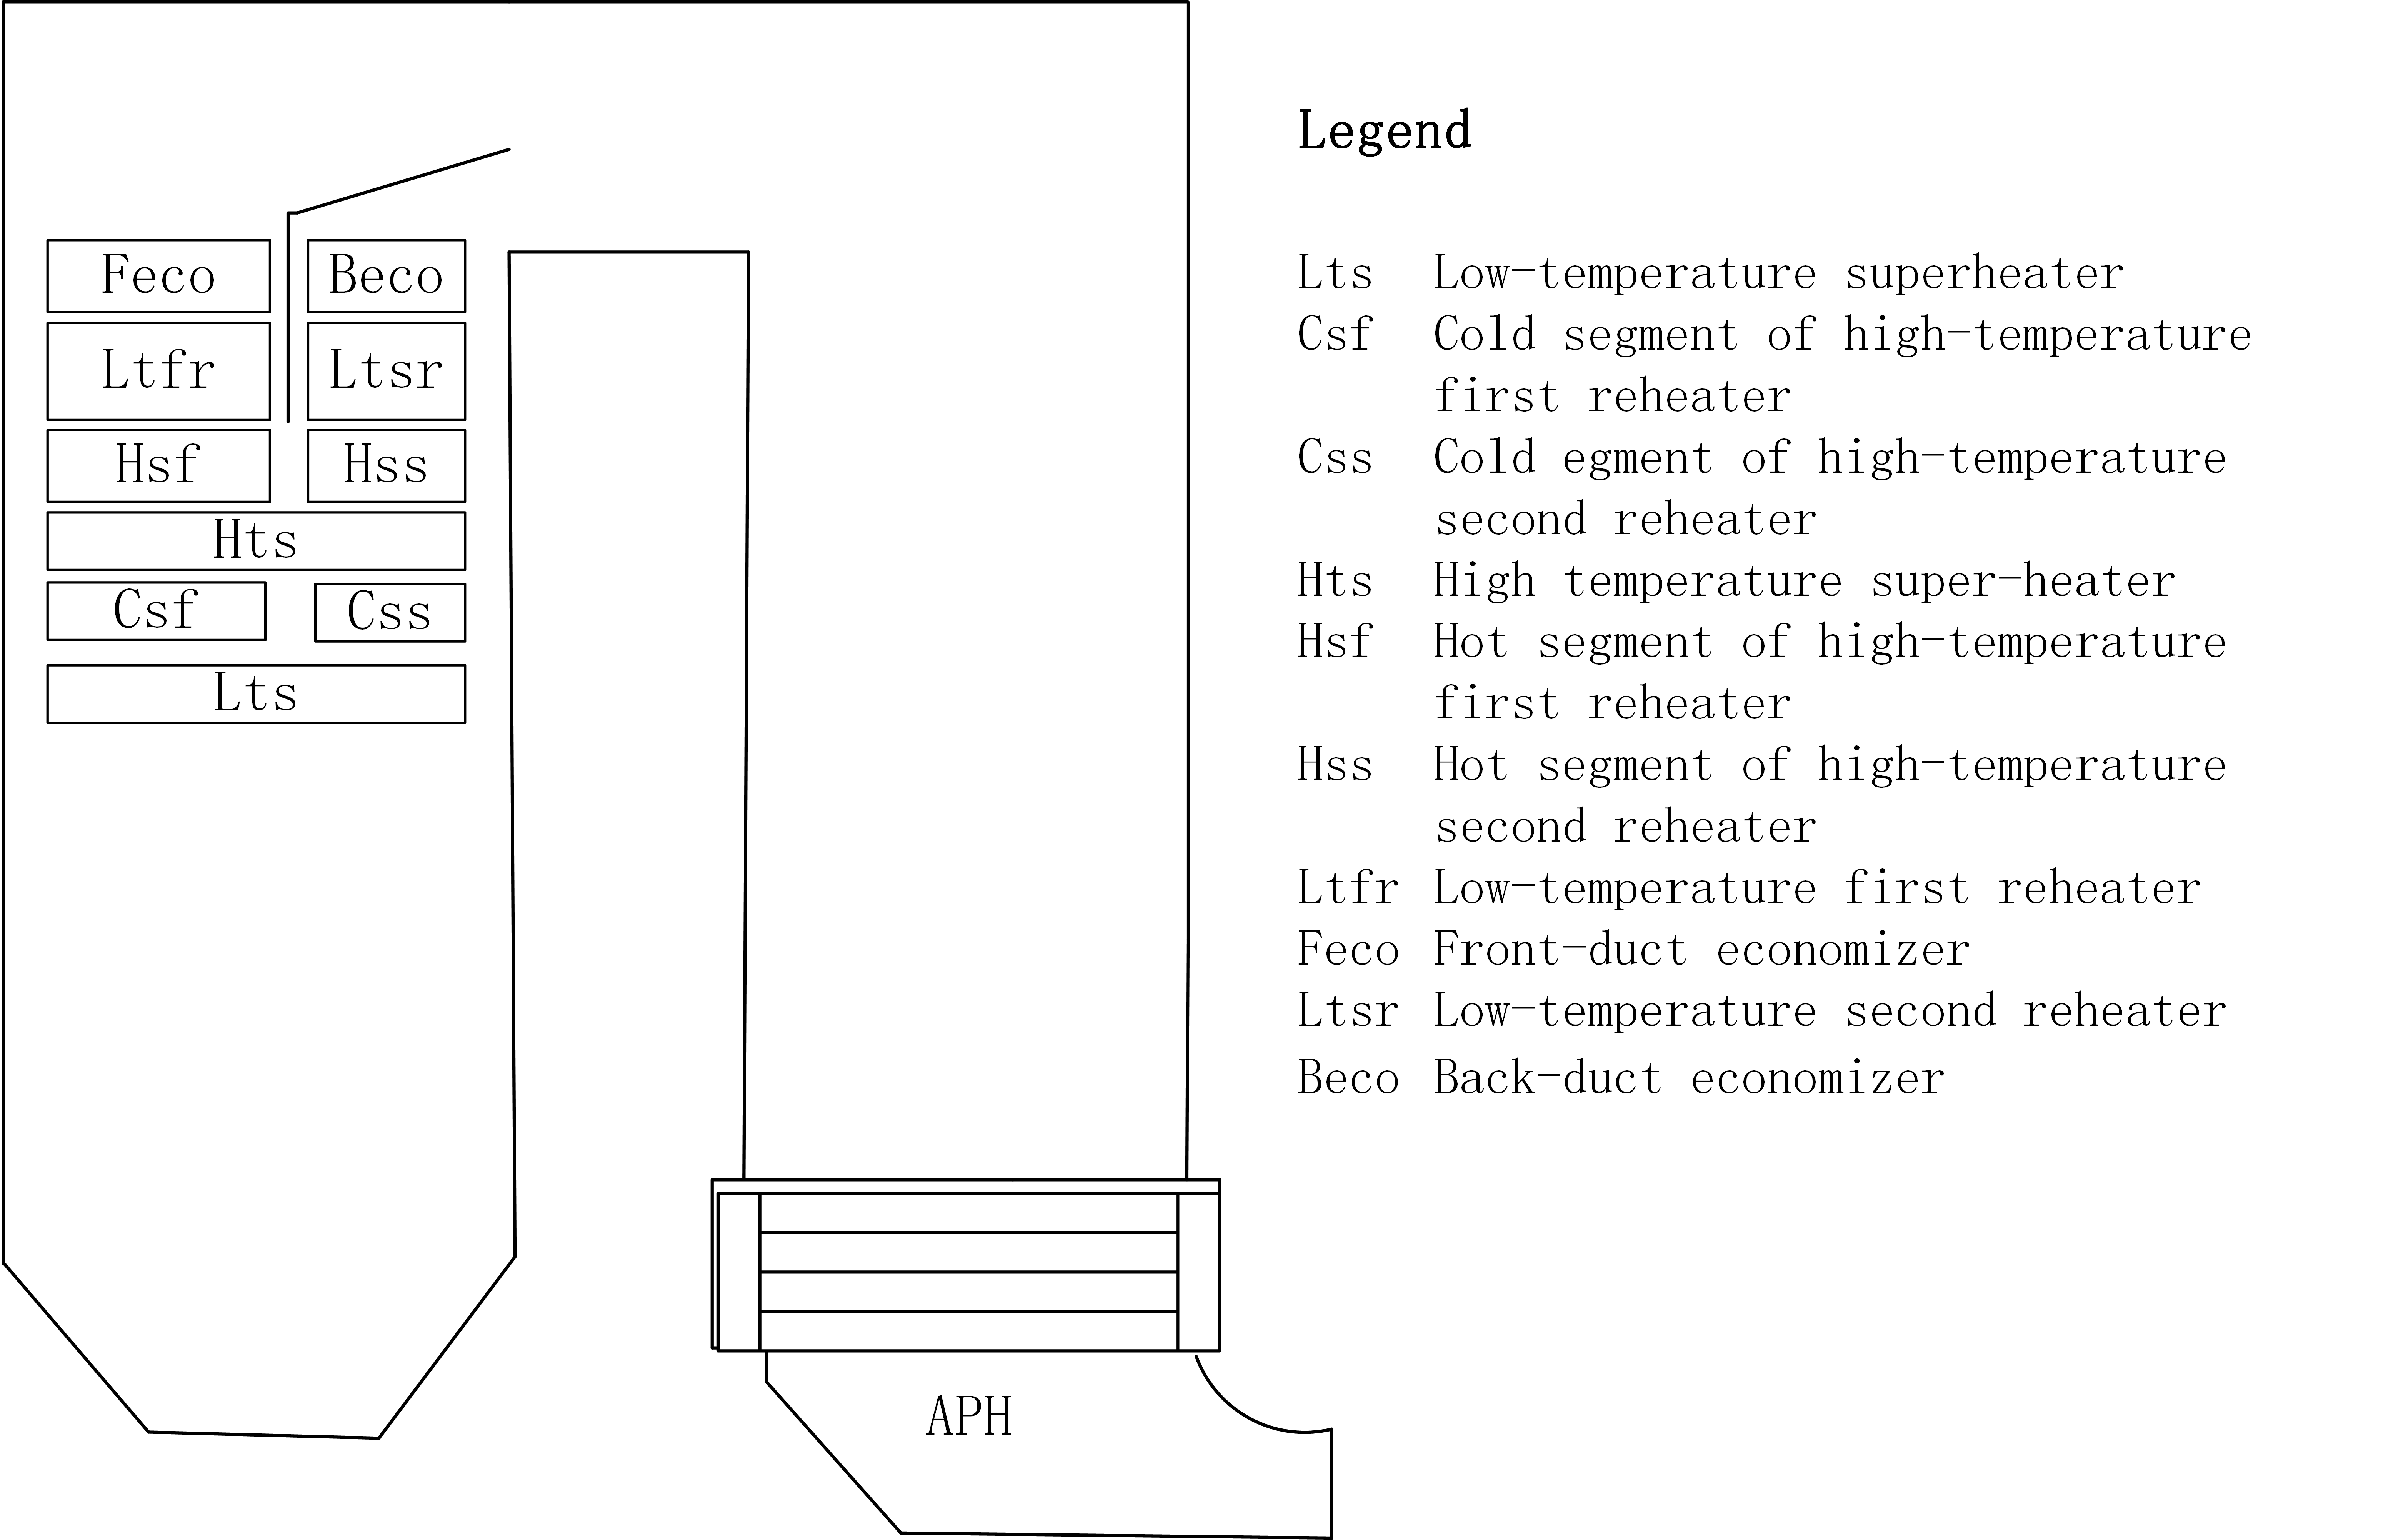
\includegraphics[width=0.9\textwidth]{fig/boiler_surface.png}
\caption{Boiler heat transfer surface layout} 
\label{fig:boiler_surface}
\end{figure}


The main parameters of the reference system are shown in Table~\ref{tab:ref input}.

\begin{table}[htbp]
\caption{Main input parameters of the reference system }
\label{tab:ref input}
\centering
\begin{tabular}{lll}
\toprule 
Items & Unit & Value\tabularnewline
\midrule
 Live steam mass flow rate 	    	&t/h 			&2533 \\
 Live steam pressure 		    	&bar 			&310\\
 Live steam temperature		     	&$^\circ$C		&600		\\
 First reheat steam pressure    	&bar			&100.9		\\
 First reheat steam temperature  	&$^\circ$C		&610		\\
 Second reheat steam pressure    	&bar			&30.8		\\
 Second reheat steam temperature 	&$^\circ$C		&610		\\
 Power generation output 			&MW				&1000		\\
\bottomrule
\end{tabular}	
\end{table}

Table~\ref{tab:reheater parameter} gives the temperature profiles of the regenerative heaters and the air preheater, revealing their energy match level.
For the APH, the temperature of the flue gas at the inlet is less than 376$^\circ$C,  
 while the temperature of the air to be heated by the flue is 23$^\circ$C.
The logarithm mean temperature difference (LMTD) of the APH is calculated as 72$^\circ$C.
Compared with the air preheater, the regenerative heaters have much lower LMTDs, ranging from 6.88$^\circ$C-15.87$^\circ$C.
According to the second law of thermodynamics, the greater the temperature difference, the greater the irreversible loss.
Therefore, the air preheat process needs to be optimized to reduce the energy loss of the system.
AOC1 and AOC2 have the same problem of high LMTDs compared with RHs.
It is important to determine how to make the double-reheat USC system's high temperature extractions a reasonable arrangement. 



\begin{table}[htbp]
\caption{Fluid parameters of regenerative heaters and air preheater} %Should "air preheater" be plural here?
\label{tab:reheater parameter}
\centering
\begin{tabular}{llll}
\toprule 
\multirow{2}{2cm}{Components} &\multirow{2}{2.7cm}{Hot fluid temperature($^\circ$C)}  & \multirow{2}{3.2cm}{Cold fluid temperature ($^\circ$C)}&\multirow{2}{2.2cm}{LMTD ($^\circ$C)}\tabularnewline
&&&\tabularnewline
\midrule
APH  &  376.00 	& 23.00  & 72.4\tabularnewline
AOC1 &   526.56 & 304.51 & 69.75\tabularnewline
AOC2 &  527.48 	& 304.51 & 60.81\tabularnewline
HRH1 &   417.07 & 273.62 & 10.64\tabularnewline
HRH2 &   314.53 & 240.73 & 10.77\tabularnewline
HRH3 &   434.54 & 205.89 & 12.68\tabularnewline
HRH4 &   316.51 & 186.48 & 6.88\tabularnewline
LRH6 &  394.01 	& 140.46 & 13.19\tabularnewline
LRH7 &   313.17 & 104.49 & 15.87\tabularnewline
LRH8 &   191.84 & 82.42  & 9.82\tabularnewline
LRH9 &   116.61 & 59.25  & 10.03\tabularnewline
\bottomrule
\end{tabular}
\end{table}




\subsection{Proposal for a novel system with EAPHs and LPEs}
\label{sub2:prop novel sys}

To reduce the energy loss caused by APH, a novel system is proposed in which air is not heated by flue gas in the conventional air preheater. Rather, eight turbine-extraction-heated air preheaters (EAPH1-EAPH8) are used.
The layout of the optimization system is presented in Fig.~\ref{fig:novel_system}.

As shown in Fig.~\ref{fig:extraction_heat_APH}, the extracted steam is divided in half, with one half sent to the regenerative heater to heat the condensate or feedwater and the other half sent to the corresponding EAPH to heat the air.
The drainage from the air preheater joins with that of the corresponding regenerative heater after the heat transfer has been completed.
The steam distribution ratio is determined according to the EAPH upper terminal temperature difference settled in the system.
It should be noted that not all of the extractions are available for air heating.
The last two stage extractions' pressure values are much lower than their barometric pressure values, which suggests a great risk of air leakage into the steam. APH8 must be shut down under low load for the same reason.

The AOCs in the reference system are designed to heat feedwater.
Although AOC inlet steam has a great supper heat degree %superheat?
, the small amount of heat exchanged makes the feedwater's temperature rise only slightly.
The LMTD is very high in AOCs.

To reduce rise AOCs' exergy efficiency and the superheat degree of extractions entering the heat exchangers,
%Here do you mean to "reduce the possibility of an increase in AOCs'..."?
four additional outer steam coolers (AOC1-AOC4) are installed at the air side outlet of EAPH1.
The air side outlet of EAPH1 is sent to the boiler as secondary air, which has a smaller mass and lower heat capacity compared with the feedwater. 
The secondary air temperature thus can increase remarkably, while the LMTD of AOCs can decrease.
The second through the fifth extractions have very high temperatures and great superheat degrees; they are sent to the AOCs in the order of their temperature levels.
For example, the second extraction has the highest temperature and is applied to heat the air in the first AOC. Then the cooled steam from AOC1 is sent to HRH2 and air EAPH2 to heat the water and air, respectively.  %Should "air EAPH2" be simply "EAPH2"?

\begin{figure}[htbp]
\centering
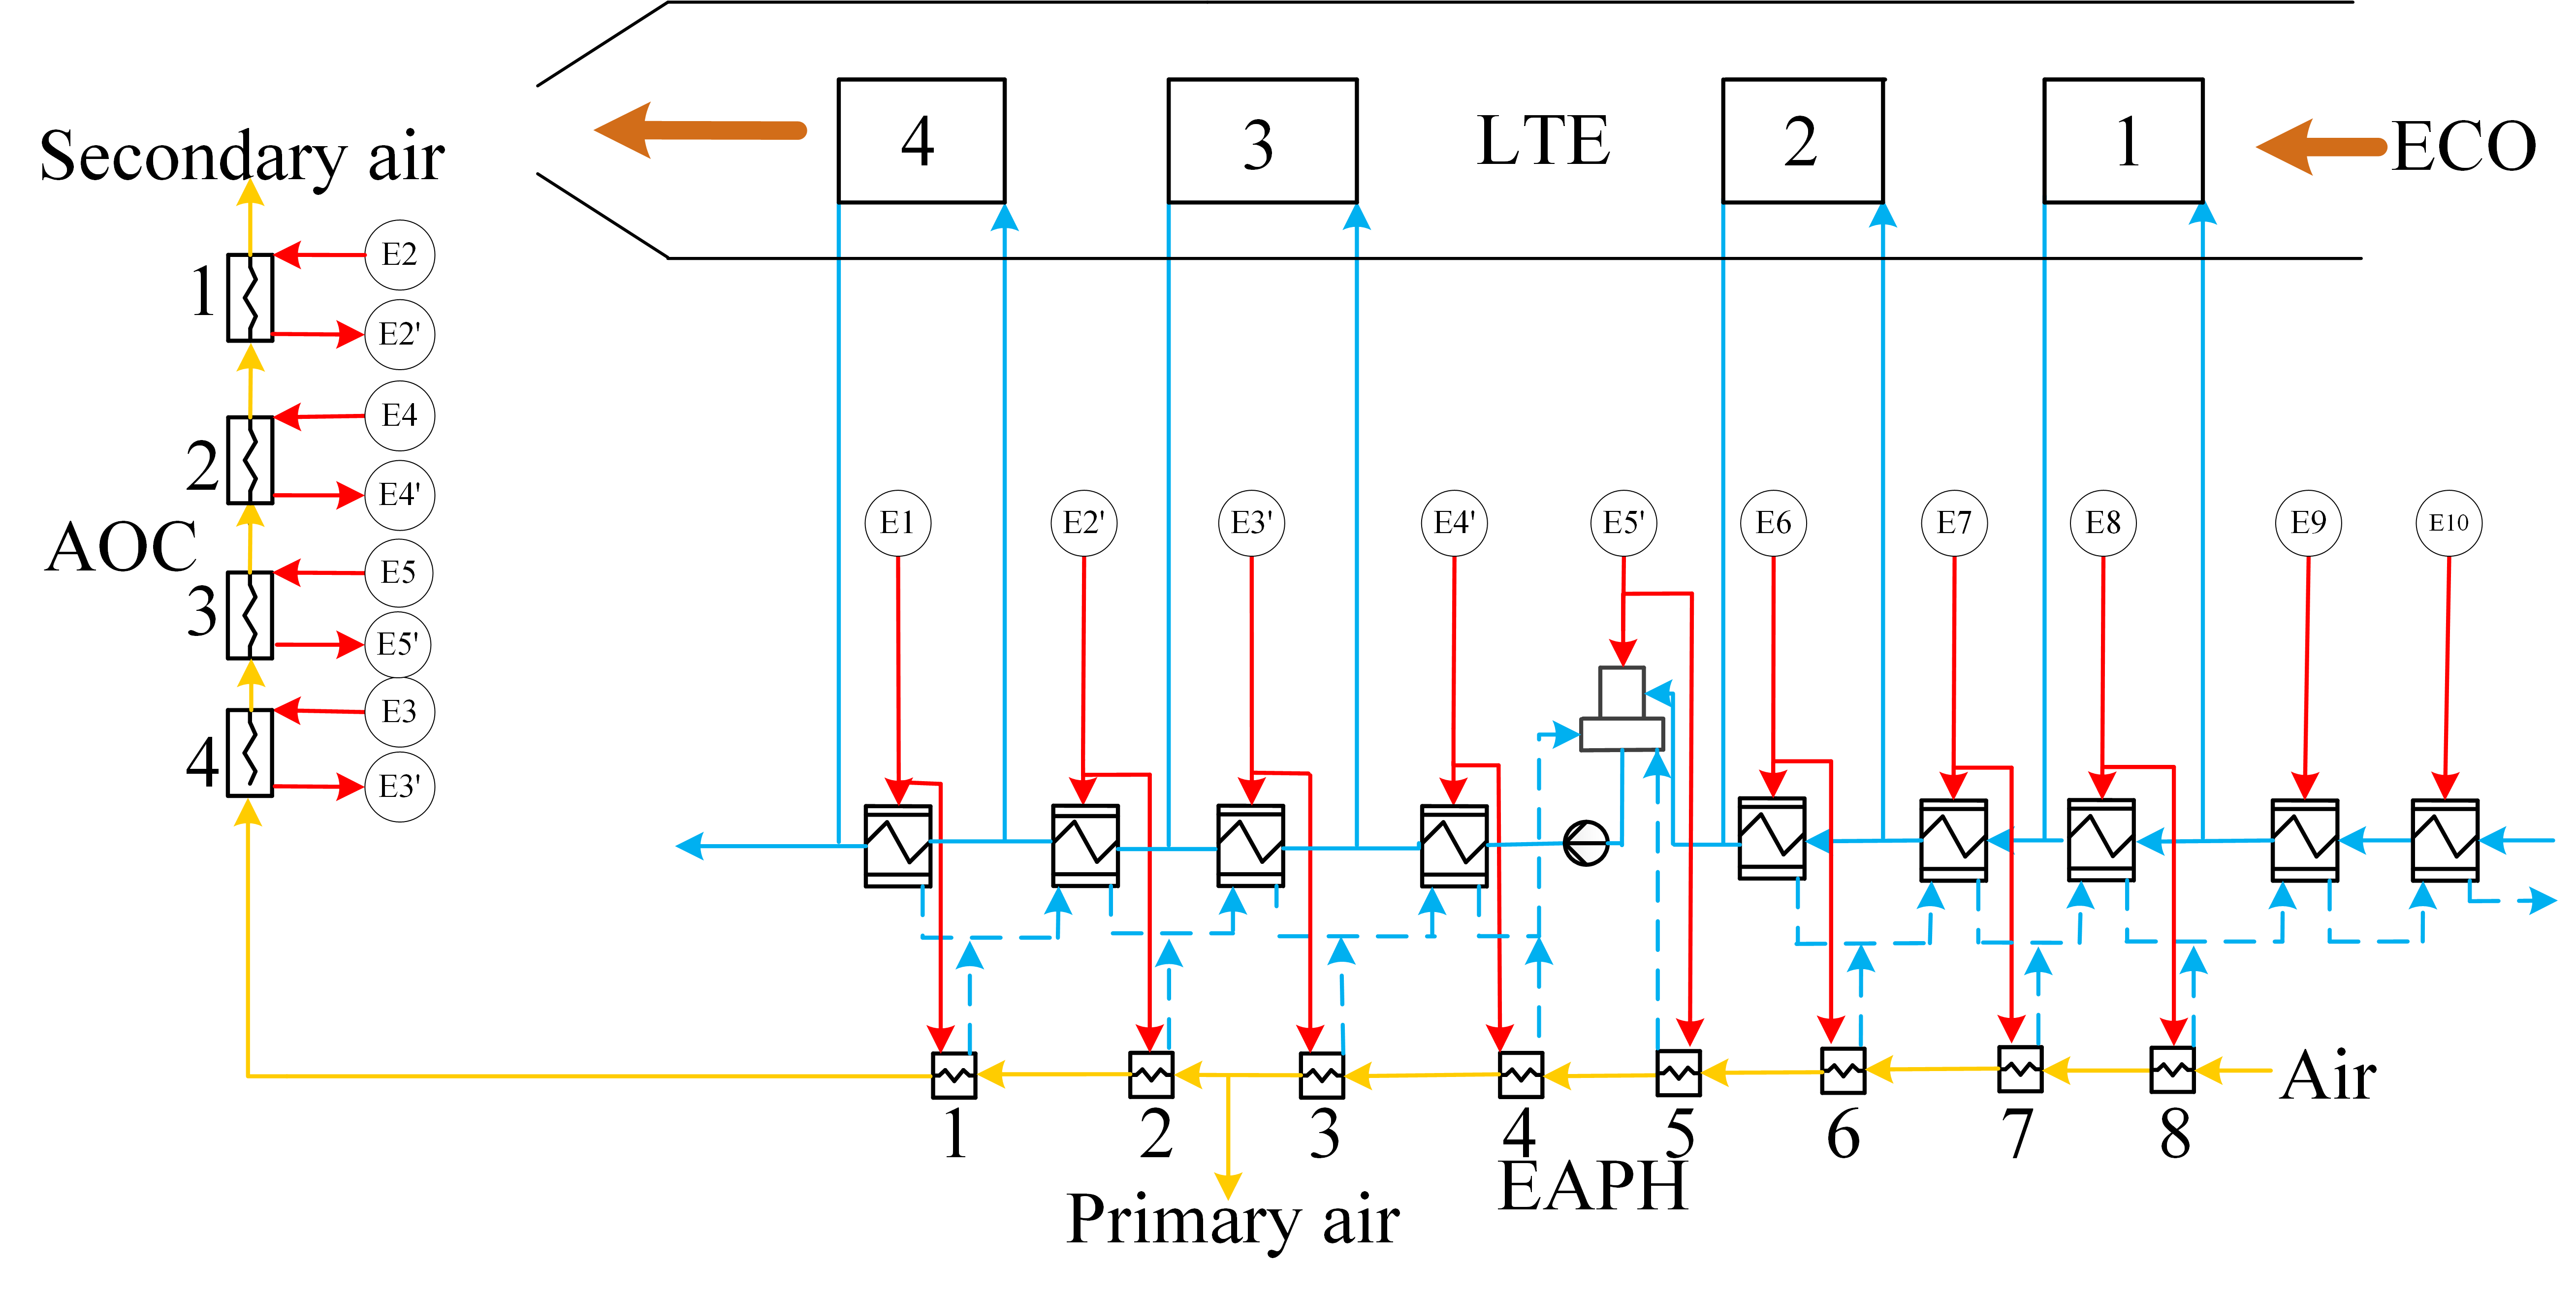
\includegraphics[width=1\textwidth]{fig/novel_system.png}
\caption{Schematic of the novel system} 
\label{fig:novel_system}
\end{figure}

\begin{figure}[htbp]
\centering
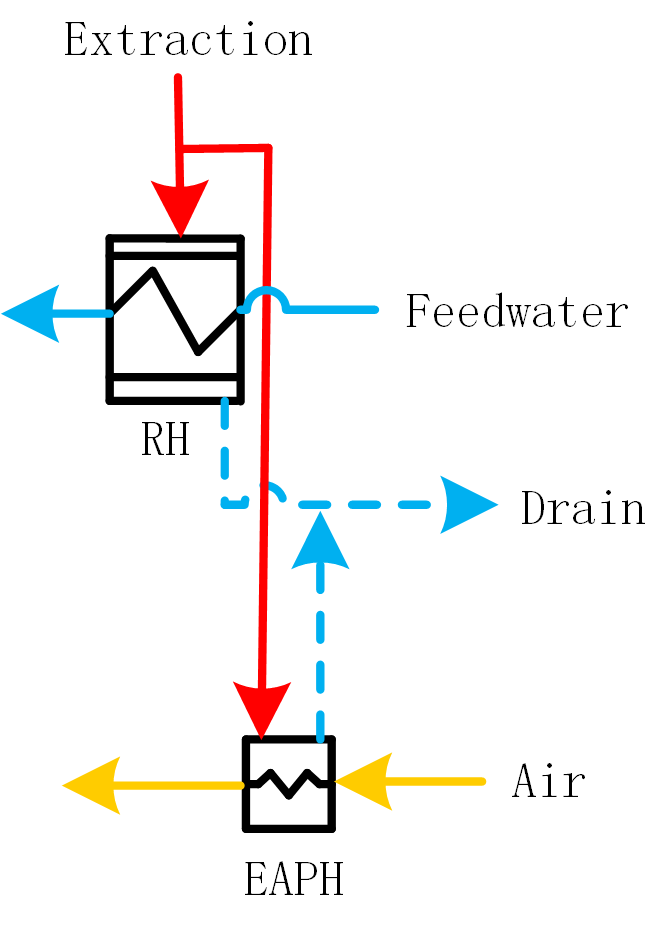
\includegraphics[width=0.3\textwidth]{fig/extracion_heat_APH.png}%extraction_heat_APH
\caption{Process flow diagram of RH and EAPH} 
\label{fig:extraction_heat_APH}
\end{figure}

Because of the removal of the APH originally installed in the vertical shaft, the flue gas's heat needs to be absorbed by other means.
As shown in Fig.~\ref{fig:novel_system}, the flue gas at the outlet of the economizer is utilized by four LPEs to heat the condensate and feedwater; these LPEs are parallel to HRH2, HRH4, LRH6, and LRH8, respectively. %Rather than "are parallel to," perhaps "correspond with"? 
Part of the condensate and feedwater at the inlet of the regenerative heater is sent to the LPE; then the heated water joins with the corresponding regenerative heater's outlet water. 
Given the acid dew point temperature, the flue gas temperature at the outlet of the last LPE can be set to 95$^\circ$C. 


% \section{Model establishment and thermodynamic evaluation} % (fold)
% \label{sec3:modle est and eval}
\section{Model description and thermodynamic metrics}
\label{ssub:model_establishment_and_system_analysis_method}

\subsection{Model establishment method and main assumptions}
\label{ssub3:modle description}
%对模型中如何基于现有系统进行的改造,和哪些数据不发生变化进行说明
%添加模型中基本部件的特性 添加个表格
In this paper, the thermodynamic cycle of the thermal system under different loads is simulated using EBSILON® Professional.
EBSILON is a power plant simulation tool that can calculate thermodynamic quantities. It is widely used in power plant system model establishment and analysis~\cite{Li2015Integrated,Yao2017Multi}. 
The simulation model yields detailed data with a high degree of reliability in calculating the thermodynamic state.
When using this software simulation system, the main equipment's work flow parameters and some basic properties need to be settled.
Because it is designed based on the reference system, the novel system's main input parameters (such as live steam parameters, first/second reheat steam parameters, and turbine extraction parameters) remain the same as those that are shown in Table~\ref{tab:ref input} and Table~\ref{table:extractions_parameter}.
Based on the practice,
%What is "the practice"? 
the upper temperature differences of the novel system's LPE, AOC and EAPH are settled to 30$^\circ$C, 20$^\circ$C, and 5$^\circ$C. 
The details of the model's other main components are given in Table~\ref{table:model_details}. 

\begin{table}
\caption{Details of model's main components}
\label{table:model_details}
\begin{centering}
\begin{tabular}{ll}
\toprule 
Components 				& Model details\tabularnewline
\midrule
Boiler         			& Economizer outlet flue gas temperature = 376\textcelsius \tabularnewline
 						& Slag temperature = 850\textcelsius \tabularnewline
 						& Combustion efficiency = 0.99\tabularnewline
Turbine 				& Isentropic efficiencies range from 0.83 to 0.93, \tabularnewline
 						& calculated from the thermal equilibrium diagram\tabularnewline
Condenser 				& Upper terminal temperature difference = 5\textcelsius \tabularnewline
Regenerative reheats 	& Upper terminal temperature differences range from -1.7\textcelsius{}  \tabularnewline
 						& to 2.2\textcelsius, calculated from the thermal equilibrium diagram.\tabularnewline
\bottomrule
\end{tabular}
\par\end{centering}
\end{table}

Under off-design conditions, EBSILON's simulation and parameter calculations for equipment such as turbines are based on the experimental characteristics of the units.
However, only the turbine's off-design characteristic curves can actually be obtained, while the data for the boiler and heat exchangers cannot be determined.
This data thus has to be replaced by built-in data.
It is necessary to assume the difference between the built-in data and the actual data to meet the error requirements.
%What assumption is being made about the difference in the line above?
The following assumptions need to be made in order to be able to correctly perform a simulation.
\begin{enumerate}[(1)]
\item Both the novel and reference systems are operated under stable conditions.
\item The thermal efficiency of the equipment is calculated from the thermal balance of the input and output parameters of the components, assuming that the calculation error requirement is met.
\item According to the heat map, the upper and lower end differences of the heat exchanger are set as fixed values and do not change during different load conditions' simulation.
\item The pips' complexity and the installation difficulty of the novel system's equipment is not taken into consideration.
\end{enumerate}
A more detailed description of the thermaldynamic model of the components can be found in Ref.~\cite{Yao2017Multi}. %Should this be "thermodynamic," rather than "thermaldynamic"?

\begin{table}
\caption{Turbine extractions' parameters under the design condition}
\label{table:extractions_parameter}
\begin{centering}
\begin{tabular}{cccccc}
\toprule 
\multirow{2}{*}{Extractions} & Pressure & Temperature & \multirow{2}{*}{Extractions} & Pressure & Temperature\tabularnewline
 & (bar) & (℃) &  & (bar) & (℃)\tabularnewline
\midrule
1st & 107.89  & 429.00 & 6th & 7.15  & 394.01 \tabularnewline
2nd & 61.89 & 528.30  & 7th & 3.90  & 313.17\tabularnewline
3rd & 34.34 & 435.20  & 8th & 1.23  & 191.84\tabularnewline
4th & 17.56  & 526.55  & 9th & 0.57  & 116.61\tabularnewline
5th & 10.35  & 447.37 & 10th & 0.21 & 62.57\tabularnewline
\bottomrule
\end{tabular}
\par\end{centering}
\end{table}

\subsection{Thermodynamic metrics} %(fold)
\label{ssub3:analsys method} 
%为了能够对优化系统与参考系统进行评估,揭示系统优化的内在机理,本文引入热力学第二定律的分析方法即用分析方法。
Based on the second law of thermodynamics, the exergy analysis method has been widely used in power plant thermal system analysis and optimization~\cite{Si2017Exergy,Yang2013Comprehensive,Ahmadi2016Energy}
Exergy analysis is adopted to reveal the location, the magnitude, and the sources of a unit's thermodynamic inefficiencies.
Exergy destruction and exergy efficiency are usually chosen as evaluation indices for the thermal system or an individual component within the system. 
The general exergy balance of a system or its component can be expressed in the following form:
\begin{equation}
\label{equation:1}
\dot{I}=\sum\dot{Ex}{}_{in}-\sum\dot{Ex}{}_{out}+\sum\dot{W}{}_{in}-\sum\dot{W}{}_{out}
\end{equation}





Exergy efficiency can be calculated using the following form:
\begin{equation}
\label{equation:2}
\eta_{\uppercase\expandafter{\romannumeral2}}=\frac{\dot{Ex}{}_{earned}}{\dot{Ex}{}_{cost}}
\end{equation}
For different equipment under stable operating conditions, Equations~\ref{equation:1} and ~\ref{equation:2} have different forms, as shown in Table~\ref{tab:exergy equation}~\cite{Aljundi2009Energy}

\begin{table}
\caption{Exergy analysis equations for power plant components}
\label{tab:exergy equation}
\centering
\begin{tabular}{lll}
\toprule 
 & Exergy destruction rate & Exergy efficiency\tabularnewline
\midrule
Boiler & $\dot{I}_{boiler}=\dot{Ex}{}_{fuel}+\dot{Ex}{}_{in}-\dot{Ex}{}_{out}$ & $\eta_{\uppercase\expandafter{\romannumeral2},boiler}=\frac{\dot{Ex}{}_{out}-\dot{Ex}{}_{in}}{\dot{Ex}{}_{fuel}}$\tabularnewline
Pump & $\dot{I}_{pump}=\dot{Ex}{}_{in}-\dot{Ex}{}_{out}+\dot{W}{}_{pump}$ & $\eta_{\uppercase\expandafter{\romannumeral2},pump}=1-\frac{\dot{I}_{pump}}{\dot{W}{}_{pump}}$\tabularnewline
Heater & $\dot{I}_{heater}=\dot{Ex}{}_{in}-\dot{Ex}{}_{out}$ & $\eta_{\uppercase\expandafter{\romannumeral2},heater}=1-\frac{\dot{I}_{heater}}{\dot{Ex}{}_{in}}$\tabularnewline
Turbine & $\dot{I}_{turbine}=\dot{Ex}{}_{in}-\dot{Ex}{}_{out}-\dot{W}{}_{el}$ & $\eta_{\uppercase\expandafter{\romannumeral2},turbine}=1-\frac{\dot{I}_{turbine}}{\dot{Ex}{}_{in}-\dot{Ex}{}_{out}}$\tabularnewline
Condenser & $\dot{I}_{condenser}=\dot{Ex}{}_{in}-\dot{Ex}{}_{out}+\dot{W}{}_{pump}$ & $\eta_{\uppercase\expandafter{\romannumeral2},boiler}=\frac{\dot{Ex}{}_{out}}{\dot{Ex}{}_{in}+\dot{W}{}_{pump}}$\tabularnewline
Cycle &$\dot{I}_{total}=\dot{Ex}{}_{fuel}-\dot{W}{}_{net,out}$ & $\eta_{\uppercase\expandafter{\romannumeral2},total}=\frac{\dot{W}{}_{net,out}}{\dot{Ex}{}_{fuel}}$\tabularnewline
\bottomrule
\end{tabular}
\end{table}

For flue gas, air, water, and steam, the specific exergy can be calculated using Equation~\ref{equation:3}.

\begin{equation}{}
\label{equation:3}
ex=h-h_{0}-T_{0}\left(s-s_{0}\right)
\end{equation}
Then the total exergy rate associated with the fluid stream becomes:
%Should "stream" be replaced by "steam"? 
\begin{equation}
\dot{Ex}=\dot{m}x=\dot{m}\left[h-h_{0}-T_{0}\left(s-s_{0}\right)\right]{}
\end{equation}
The fuel-specific exergy calculation method~\cite{Yan2016The} can be expressed as:
\begin{equation}
ex_{fuel}=LHV\left(1.0064+0.1519\frac{H}{C}+0.0616\frac{O}{C}+0.0429\frac{N}{C}\right)
\end{equation}
where LHV refers to the lower heating value of fuel, and C, H, O, and N refer to the mass fractions of carbon, hydrogen, oxygen, and nitrogen according to element analysis.
More details about the power plant equipment's exergy efficiency calculation can be found in Ref.~\cite{G2016Exergy}

In order to clearly analyze the effects of system optimization, this paper divides the double-reheat USC system into four main subsystems, while all other equipment, valves, and pips is together labeled "other."
The four main subsystems are the boiler without APH, the turbine, the air preheat subsystem, and the regenerative subsystem.
The equations mentioned above can be used to perform exergy analyses of these four main subsystems.
For the "other" category, this paper used a counterbalance analysis method to calculate the exergy destruction rate. This meant subtracting the share of the four main subsystems from the total exergy destruction.
The exergy destruction rate can be calculated as follows:

\begin{equation}
\dot{I}_{other}=\dot{I}{}_{total}-\sum\dot{I}{}_{subsystems}
\end{equation}


\section{Thermodynamic performance evaluation} % (fold)
\label{sub:Thermodynamic_evaluation}
%对word版本的分布进行了较大的改动,需要继续调节
\subsection{Thermodynamic comparison under design condition}
\label{ssub:desing_compare}
%表四
The comparison of the thermal dynamic performances of these two systems is given in Table~\ref{table:thermal performance compare}. %Should this be "thermodynamic" rather than "thermal dynamic"? 
Under the design condition, the novel system yields an improvement in net generating power of 11.02 MW and reduces SCE consumption by 5.5\,g/kWh.
Power generation efficiency reaches 48.73\%, which is 1.04\% higher than that of the reference system.
Meanwhile, the exergy efficiency of the novel system is 1.01\% higher, showing a good exergy-saving effect.
%"higher than that of the reference system"?

\begin{table}
\caption{Thermodynamic performance of reference and novel systems}
\label{table:thermal performance compare}
\centering
\begin{tabular}{p{7.5cm}p{1.75cm}p{1.75cm}}
\toprule 
Items & Reference system & Novel system\tabularnewline
\midrule
Net generating power (MW) & 999.10 & 1011.19\tabularnewline
Generating efficiency (\%) & 47.69 & 48.73\tabularnewline
Addition in generating efficiency (\%) &  & 1.04\tabularnewline %"Increase" rather than "Addition"? 
Standard coal consumption rate (g/kWh) & 257.59 & 252.10\tabularnewline
Reduction in standard coal consumption rate (g/kWh) &  & 5.49\tabularnewline
Exergy efficiency (\%) & 46.51 & 47.52\tabularnewline
Increase in exergy efficiency (\%) &  & 1.01\tabularnewline
\bottomrule
\end{tabular}
\end{table}
% 根据用损失对比表从新进行分析,从为什么锅炉空预器效率提高,其他不变或者降低说起
Table~\ref{table:system exergy campare} shows the results of the subsystem exergy analysis of the two systems. 
It was found that the novel system yields an improvement in exergetic performance by a decrease of 10.82\,MW in the total exergy destruction rate.
The exergy destruction rate of the boiler accounts for the highest proportion and decreases most (11.04\,MW). %Highest proportion of what? Decrease of what?
The air preheat subsystem's exergy destruction rate changes from 27.39\,MW to 16.55\,MW, having a 10.84\,MW decrement and the largest optimization ratio. %What is "decrement"?
In the meantime, the turbine and regenerative subsystem experience a relatively small change at about 1\,MW.  %Do they each have a change or do they together have one change?

The "other" category of the novel system is higher
%higher in what?
than that of the reference system, showing that the uncalculated components of systems have an increment of exergy destruction rate. %What is "an increment of exergy destruction rate"?
Among the uncalculated components, the pips' increase and parameters unmatched work fluid mixing
%I'm not sure what "parameters unmatched work fluid mixing" means---clarify?
are the main reasons that that part has an increment in exergy destruction rate.

\begin{table}
\caption{Exergy destruction rate comparison for reference and novel systems }
\label{table:system exergy campare}
\centering
\begin{tabular}{lll}
\toprule 
Items & Reference system\,(MW) & Novel system\,(MW)\tabularnewline
\midrule 
Boiler (without AP) & 883.26 & 872.22\tabularnewline
Turbine & 63.33 & 63.97\tabularnewline
Air preheat subsystem  & 27.39 & 16.55\tabularnewline
Regenerative subsystem & 22.53 & 21.56\tabularnewline
Other & 131.03 & 142.42 \tabularnewline
Total & 1127.54 & 1116.72\tabularnewline
\bottomrule
\end{tabular}
\end{table}

% 下面两段话需要根据图修改

%本文是针对空预系统和回热系统的联合优化改造,所以本文将新系统和参考系统中的差变化,系统中设备的效率和用损变化进行了分析。
To gain an in-depth understanding of both systems, a study of the main optimized subsystems, the air preheat subsystem, and the regenerative subsystem, was conducted.
Table~\ref{table:extraction_compare} shows the variations in the mass flow rates of extractions.
As illustrated in Table~\ref{table:extraction_compare}, the mass flow rates of the first, third, fifth, and eighth extractions of the novel system were greater than those of the reference system, and the rest of the extractions, with the exception of the final two, showed the opposite variation.
%What does "the opposite variation" mean?
Thus, the impact of system optimization on extraction is twofold: air is heated by extractions, which causes an increment in mass flow, and the use of LPE can save extractions so the total extraction mass flow remains nearly unchanged. %What does it mean to "save extractions"? 

The sum of the increase in mass flow for the fourth to tenth extractions ranges from 138.46 kg/s to 145.07 kg/s, while the eighth extraction increases by 13.9 kg/s.
The mass flow increase for the low-pressure extractions implies that the novel system can modify the quantity distribution of extractions.

%新系统优化可二次再热后蒸汽的抽汽,使8th抽汽量增加
\begin{table}
\caption{Extraction comparison between reference and novel systems}
\label{table:extraction_compare}
\begin{centering}
\begin{tabular}{llll}
\toprule 
\multirow{2}{*}{Extractions} & \multirow{2}{2.5cm}{Reference system (kg/s)} & \multicolumn{2}{c}{Novel system (kg/s)}\tabularnewline
\cmidrule{3-4} 
 &  & to RHs & to APHs\tabularnewline
\midrule
1st & 54.47 & 43.79 & 15.42\tabularnewline
2nd & 52.18 & 18.52 & 13.5\tabularnewline
3rd & 37.86 & 31.71 & 14.62\tabularnewline
4th & 20.53 & 5.66 & 9.5\tabularnewline
5th & 11.95 & 9.78 & 5.67\tabularnewline
6th & 19.94 & 9.88 & 7.83\tabularnewline
7th & 30.19 & 14.16 & 12.85\tabularnewline
8th & 16.31 & 3.11 & 27.1\tabularnewline
9th & 18.93 & 18.93 & 0\tabularnewline
10th & 20.61 & 20.6 & 0\tabularnewline
Total & 282.97 & 176.14 & 106.49\tabularnewline
\bottomrule
\end{tabular}
\par\end{centering}
\end{table}

Air is heated by the EAPHs and AOCs in the novel system from 23$^\circ$C to 363.33$^\circ$C. 
A majority of the outlet air of EAPH6 is sent to miler as primary air, and the rest of the air is heated to 363.33$^\circ$C. %What does "miler" mean?
Fig.~\ref{fig:APH_temper_compare} shows the air preheat process's temperature difference between the hot and cold fluid of the novel and reference systems.
The red triangle and the red hollow triangle instead for the average steam temperature of EAPH and AOC.
%I'm not sure what "instead" means in the above sentence. Could you clarify?
In order to simplify the diagram, the saturate temperature of steam instead of the EAPH's average temperature can be used. The mean temperature of the inlet and outlet should be used as the AOC's average temperature.
The figure indicates that the temperature difference of EAPHs is lower than that of APH, which suggests an improvement in exergy efficiency.
The AOCs' temperature difference is high, but as the heat exchange is relatively small, so is the exergy destruction. 
Therefore, the air preheat subsystem of the novel system has a lower exergy destruction rate and improved exergy efficiency.
On the other hand, the total heat exchange and secondary air temperature of the novel system are higher than those of the reference system, which indicates improvement in the boiler's exergy efficiency.

\begin{figure}[htbp]
\centering
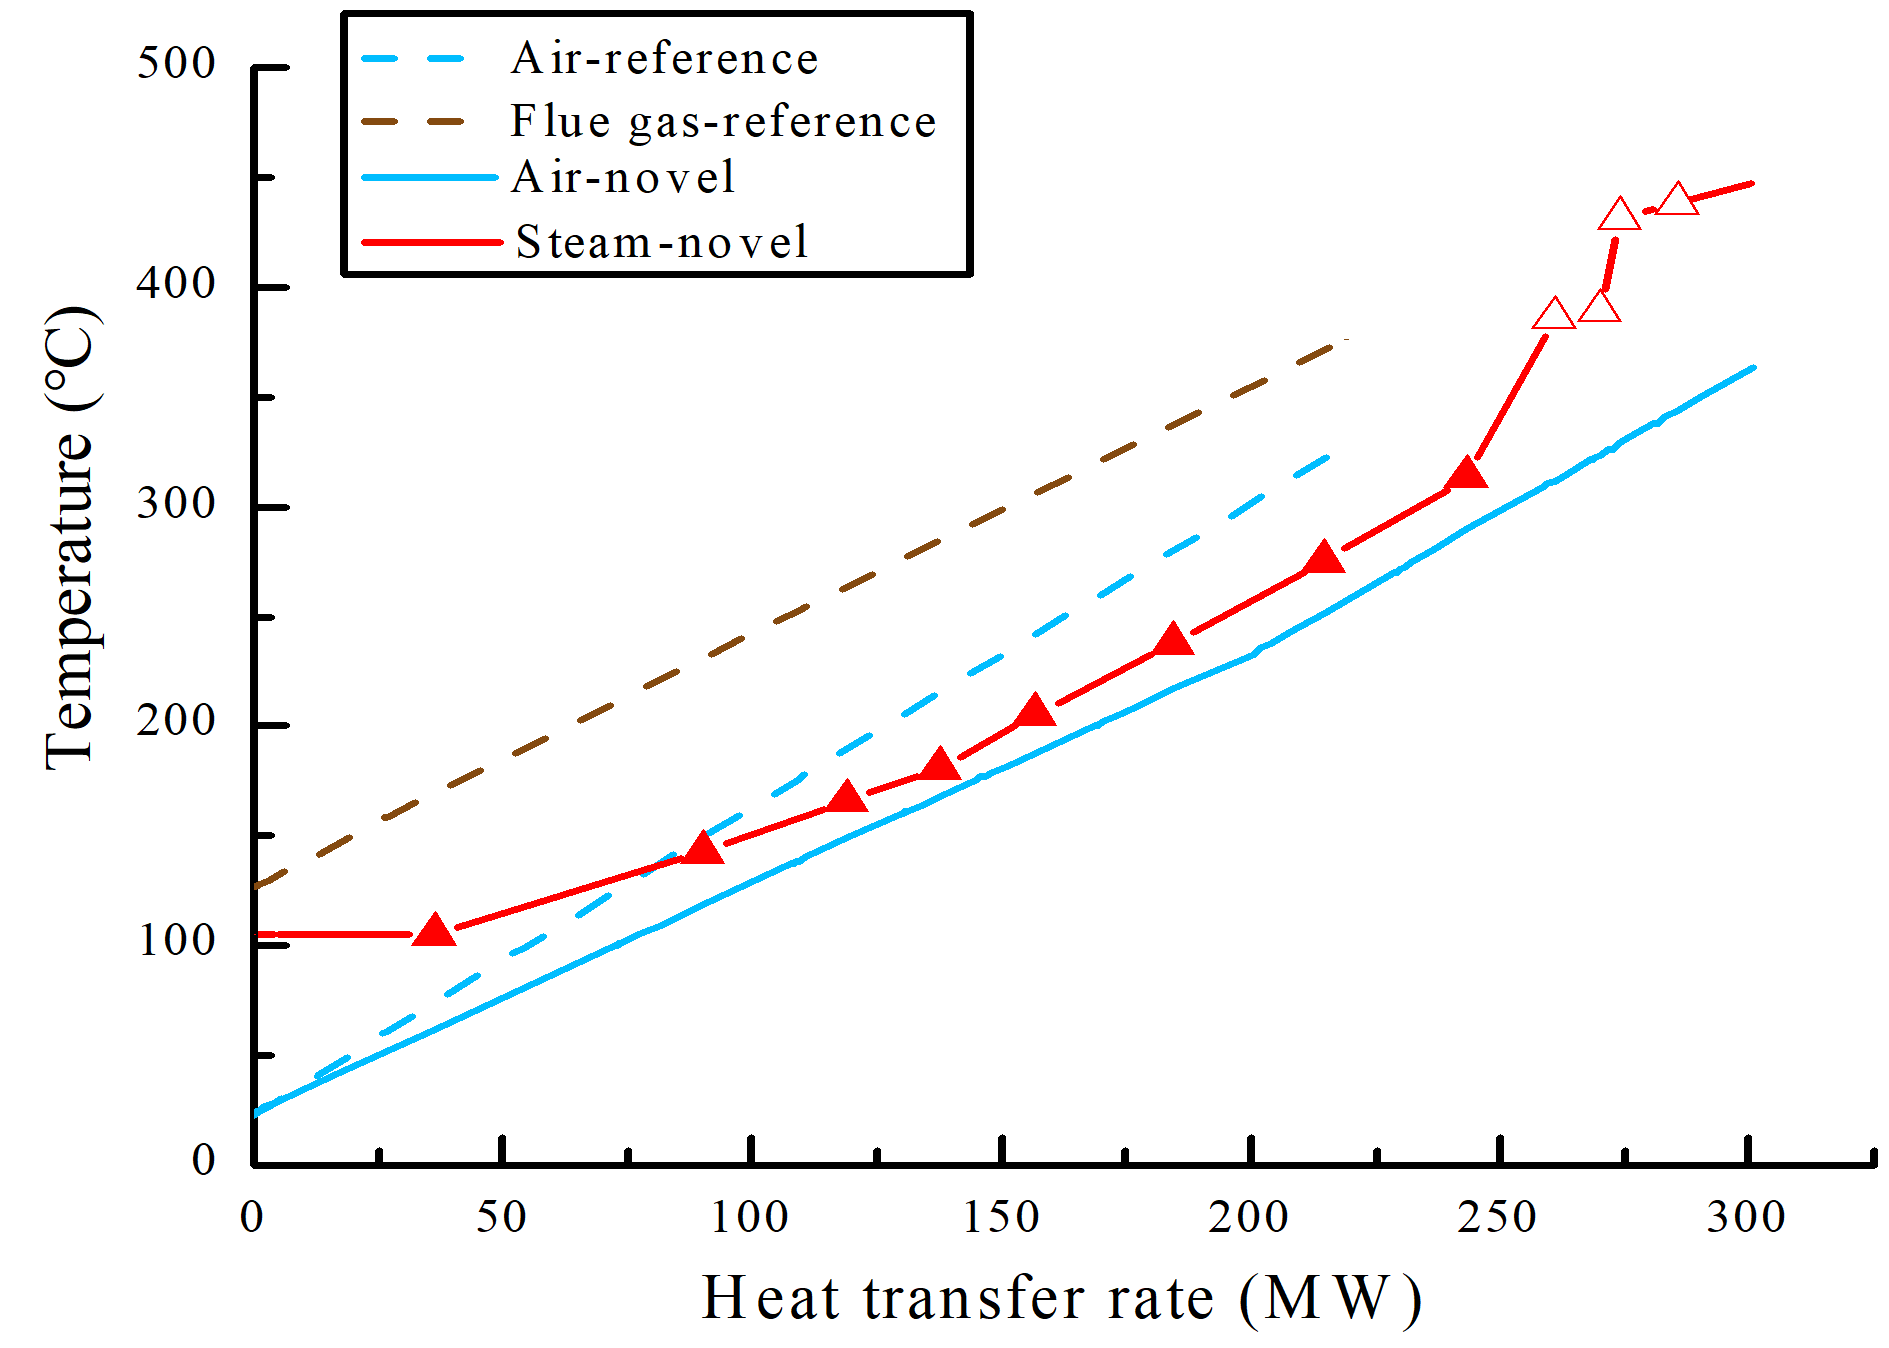
\includegraphics[width=0.6\textwidth]{fig/APH_temper_compare.png}
\caption{T-Q diagram of air preheat subsystems} 
\label{fig:APH_temper_compare}
\end{figure}


Fig.~\ref{fig:APH_temper_compare} shows EAPHs and AOCs' exergy analysis results. 
With the exception of EAPH8,the EAPHs and AOCs have exergy efficiency values higher than 82\%. APH8 has the greatest exergy loss and lowest efficiency of all the air preheaters. 
According to Fig.~\ref{fig:APH_temper_compare}, the heat transfer temperature difference of EAPH8 is 26.95 $^\circ$C,and EAPH8 has a greater heat exchanging quantity, both of which cause higher exergy destruction and exergy efficiency.
%Less exergy efficiency?
This also indicates that although the AOCs have a large heat transfer temperature difference, their exergy efficiencies are still high and their exergy destruction rates are low.

Combining Fig.~\ref{fig:APH_temper_compare} and Fig.~\ref{fig:novel_APH_exergy}, we can see that the reason that the novel system's air preheat subsystem
%Should this be "subsystems," plural?
have a higher exergy efficiency and lower exergy destruction rate is that the novel system's air preheat subsystem has a lower heat transfer temperature difference and reasonable extractions' superheat degree using.
%I'm not sure what the final part of this sentence means. What is "reasonable extractions' superheat degree using"? Is there a word missing?


\begin{figure}[htbp]
\centering
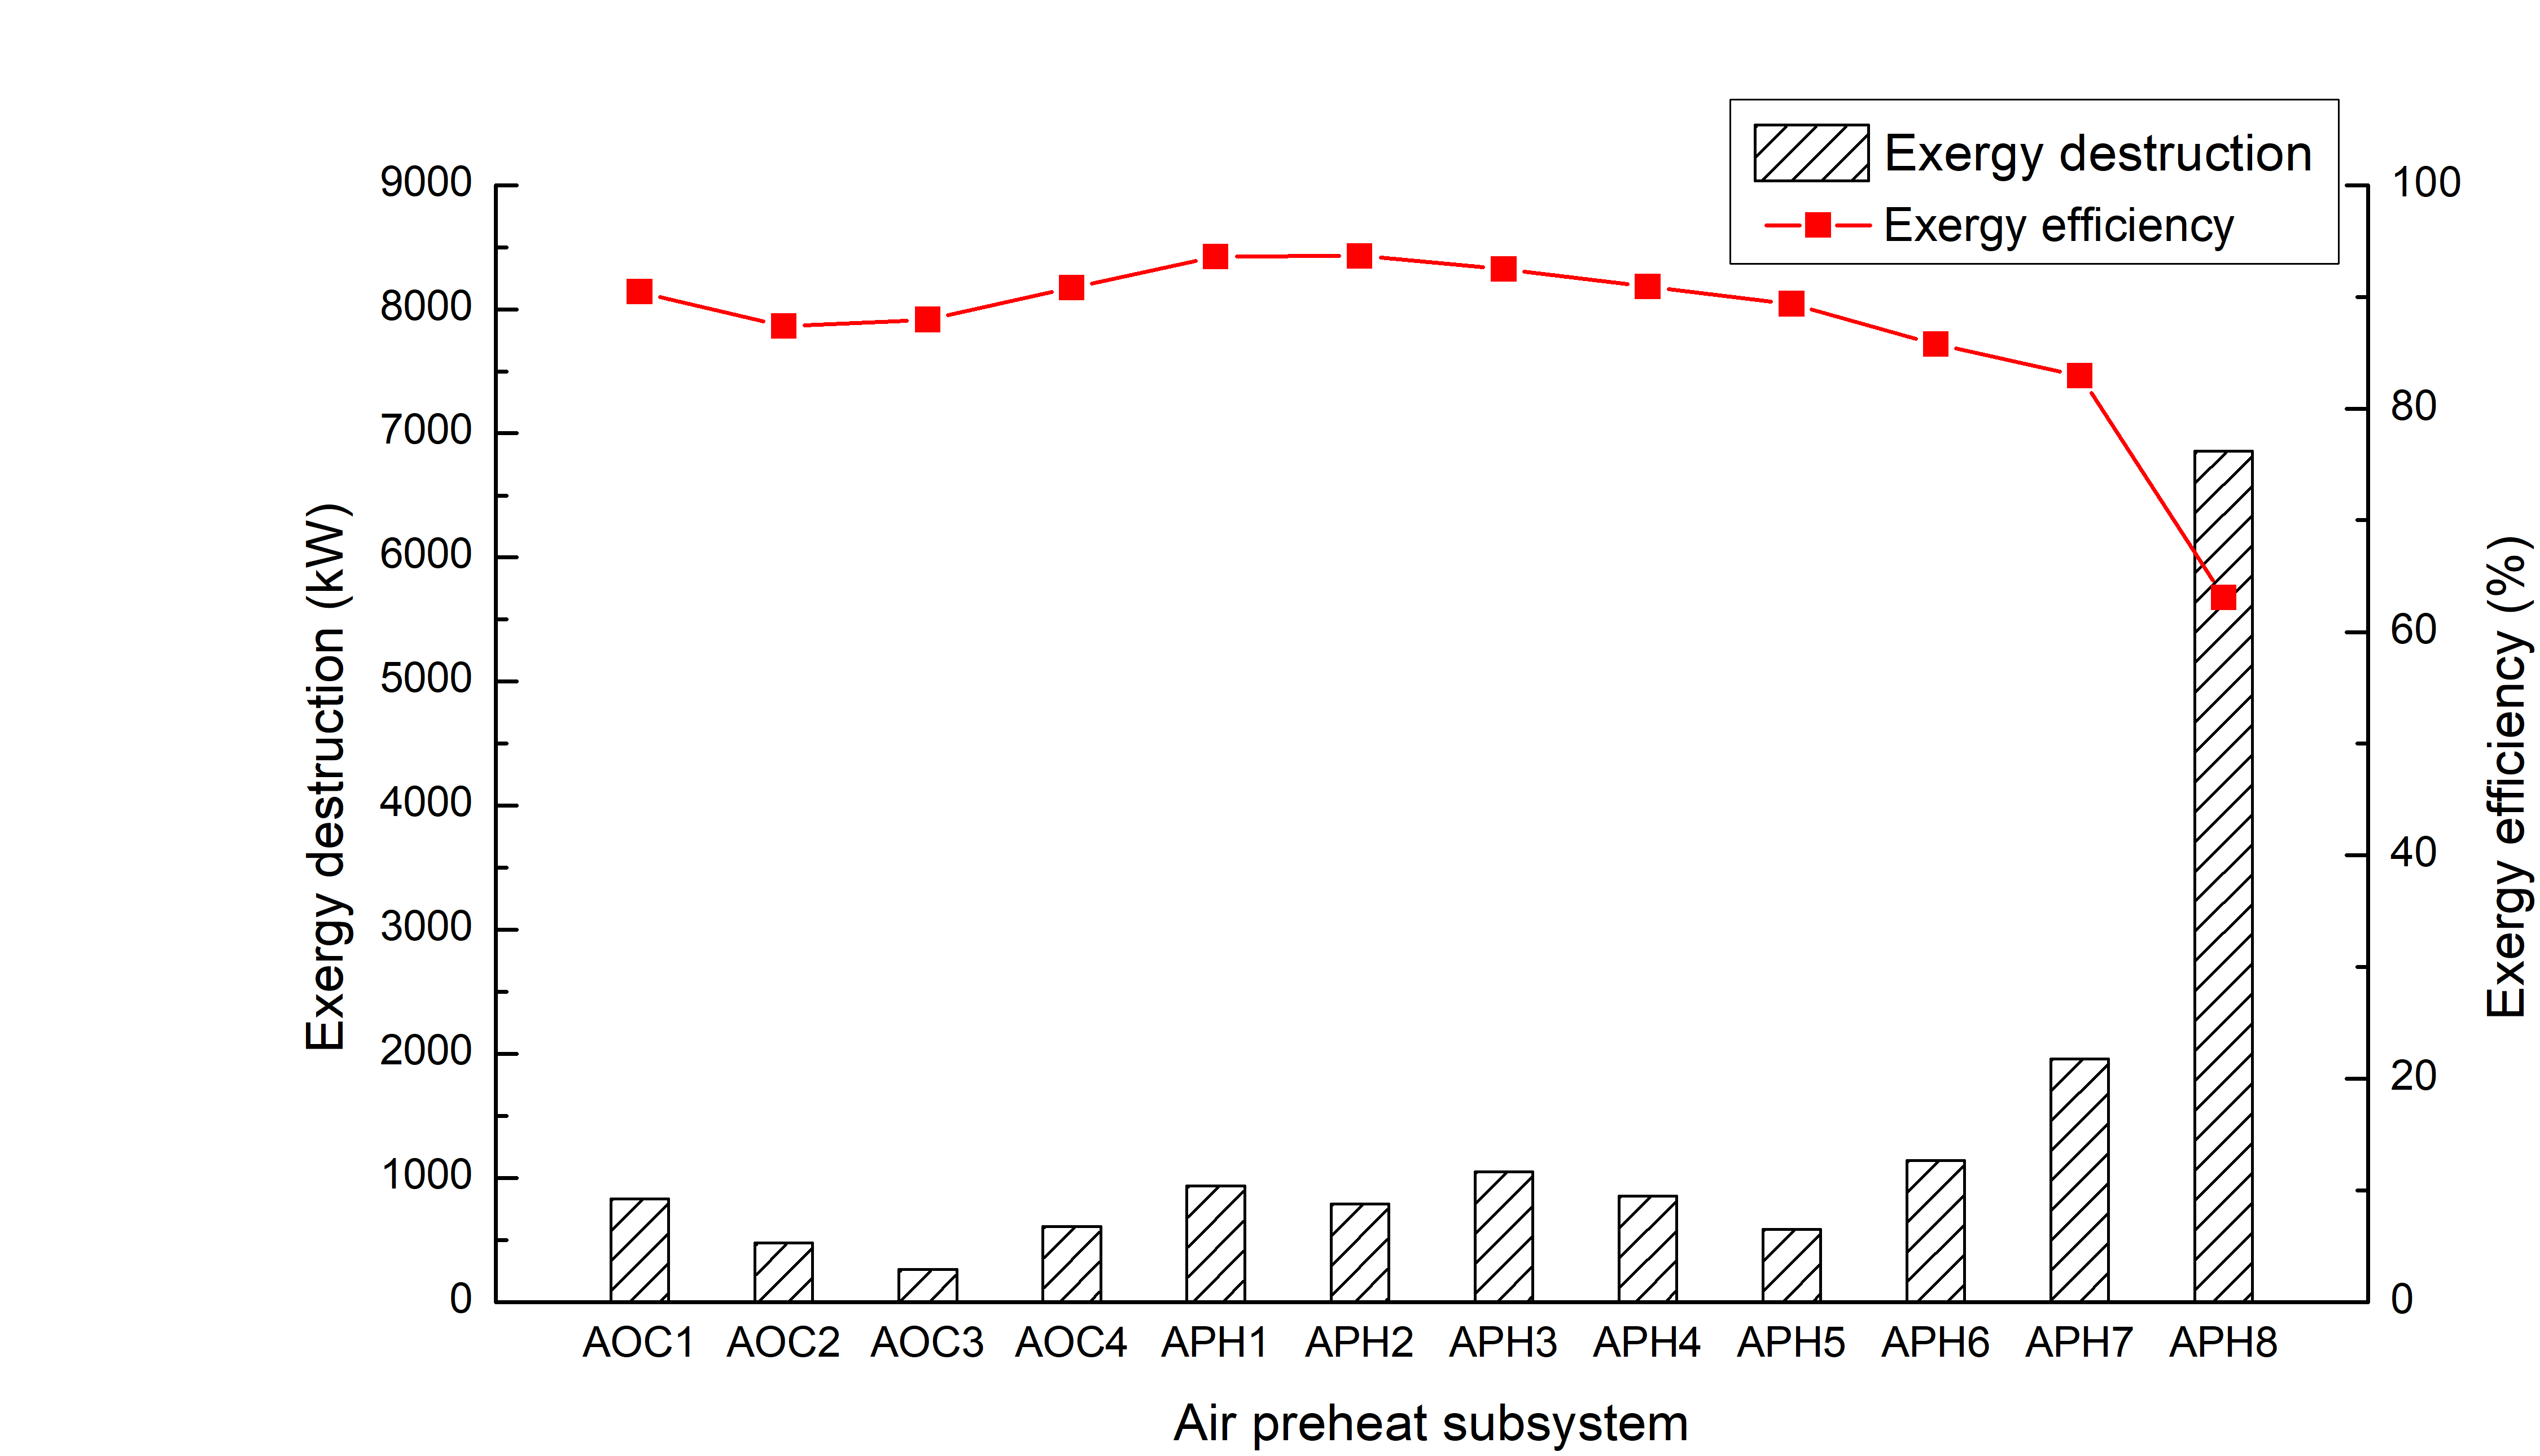
\includegraphics[width=0.8\textwidth]{fig/novel_APH_exergy.png}
\caption{Exergy destruction and efficiency of the novel system's air preheat subsystem} %图中的纵坐标需要修改
\label{fig:novel_APH_exergy}
\end{figure}

The regenerative subsystem of the novel system uses LEPS
%Should this be "LPEs"? Or if this is a new acronym, write out on first usage.
paralleled connected with EAPH to absorb the economizer's outlet flue heat and eliminate the AOCs originally used to heat feedwater.
%What does "paralleled connected" mean?
LPE inlet water is heated to the temperature of the corresponding RH outlet temperature of to mix up.
%What does "of to mix up" mean?
Keeping the extractions' parameters constant, the average heat transfer temperature difference of the RHs changes little.
This means that their exergy efficiency is the same as that of the reference system.

Fig.~\ref{fig:regenerative_subsys_compare} shows the regenerative subsystem's exergy destruction rate distribution between the two systems.
It can be seen that the novel system's exergy destruction rate decreased and great changes have taken place in the destruction's distribution.
Because of the flow-diverting effects of LEPs,%LPEs?
the exergy destruction rate of regenerative reheaters and DEA changes from 20.16 MW to 11.303 MW.
%What does "DEA" stand for?
The LEPs' %LPEs?
exergy destruction rate reaches 10.25 MW, and Fig.~\ref{fig:LPE_exergy_LMDT} shows the LEPs'
%LPEs?
exergy efficiency and heat transfer LMTD.
As shown in Fig.~\ref{fig:LPE_exergy_LMDT}, the highest efficiency one is LPE1 with 93.50\%, and the lowest efficiency one is LPE4 with 87.44\%. 
The LEPs'
%LPEs'?
overall exergy efficiency is 91.62\%, which is much higher than that of the flue-air heat transfer of the reference system, and the temperature difference of the LPEs is between 23$^\circ$C and 42$^\circ$C.

\begin{figure}[htbp]
\centering
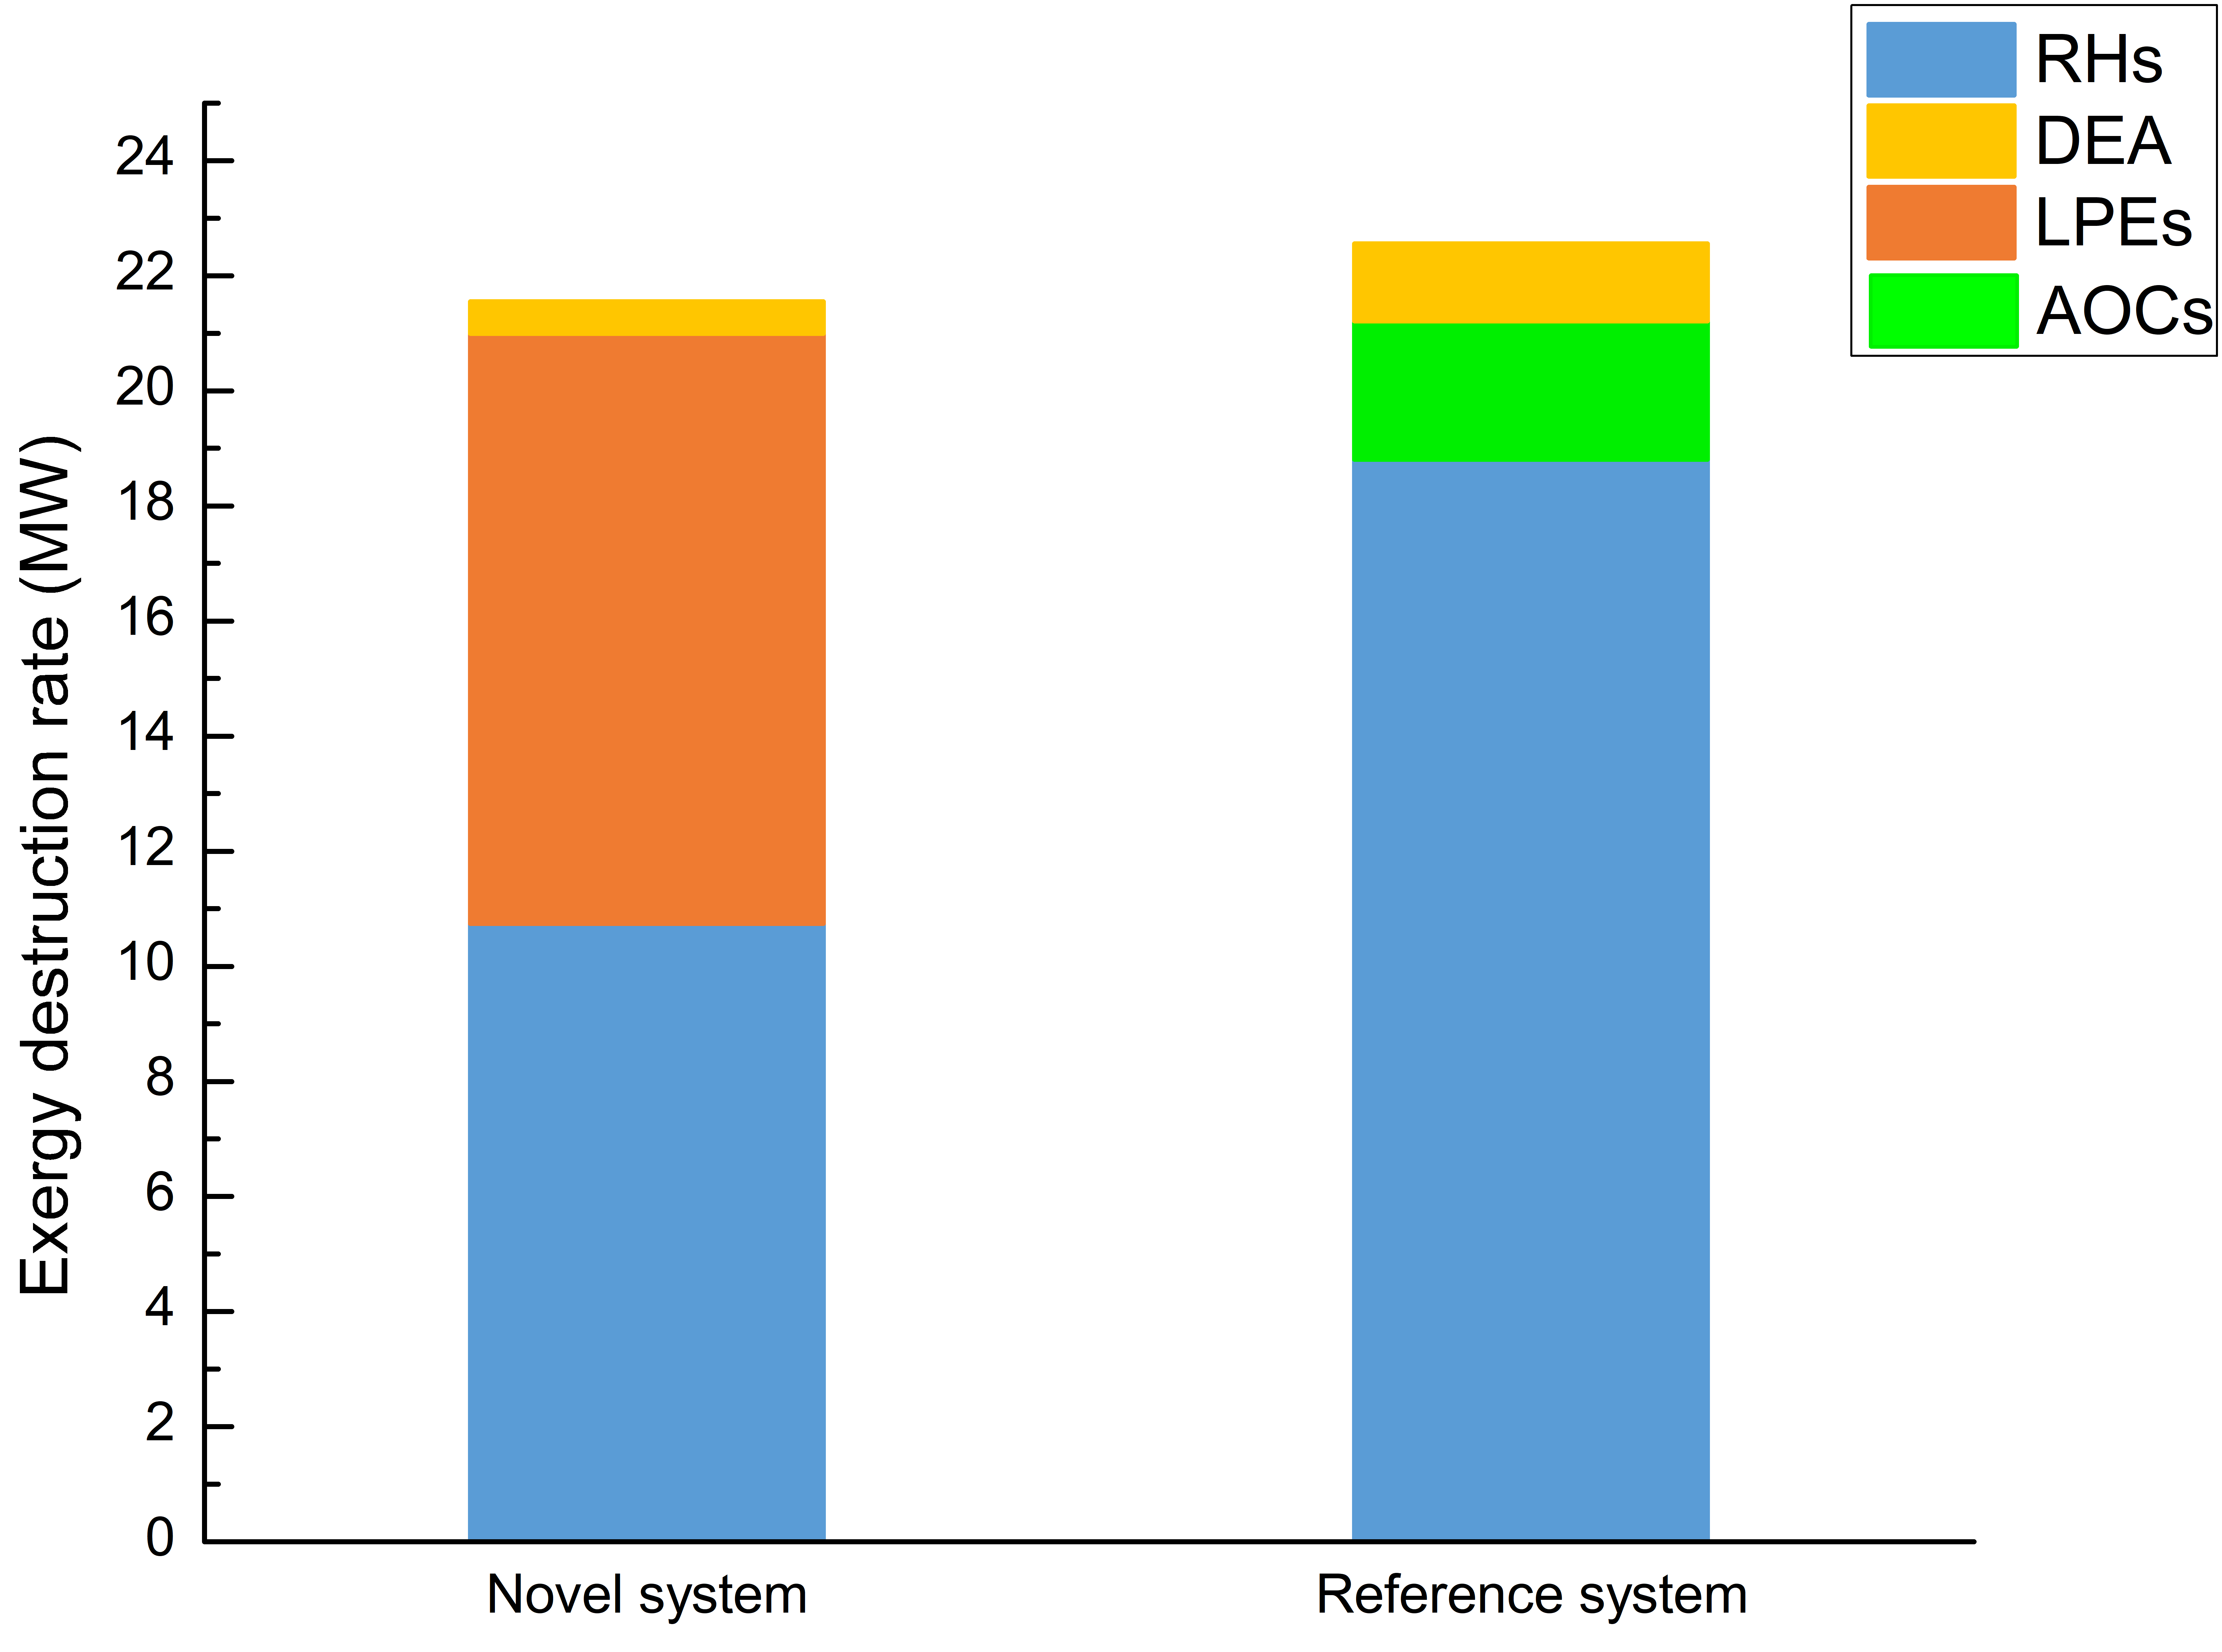
\includegraphics[width=0.6\textwidth]{fig/regenerative_subsys_compare.png}
\caption{Exergy destruction comparison of regenerative subsystems} 
\label{fig:regenerative_subsys_compare}
\end{figure}



\begin{figure}[htbp]
\centering
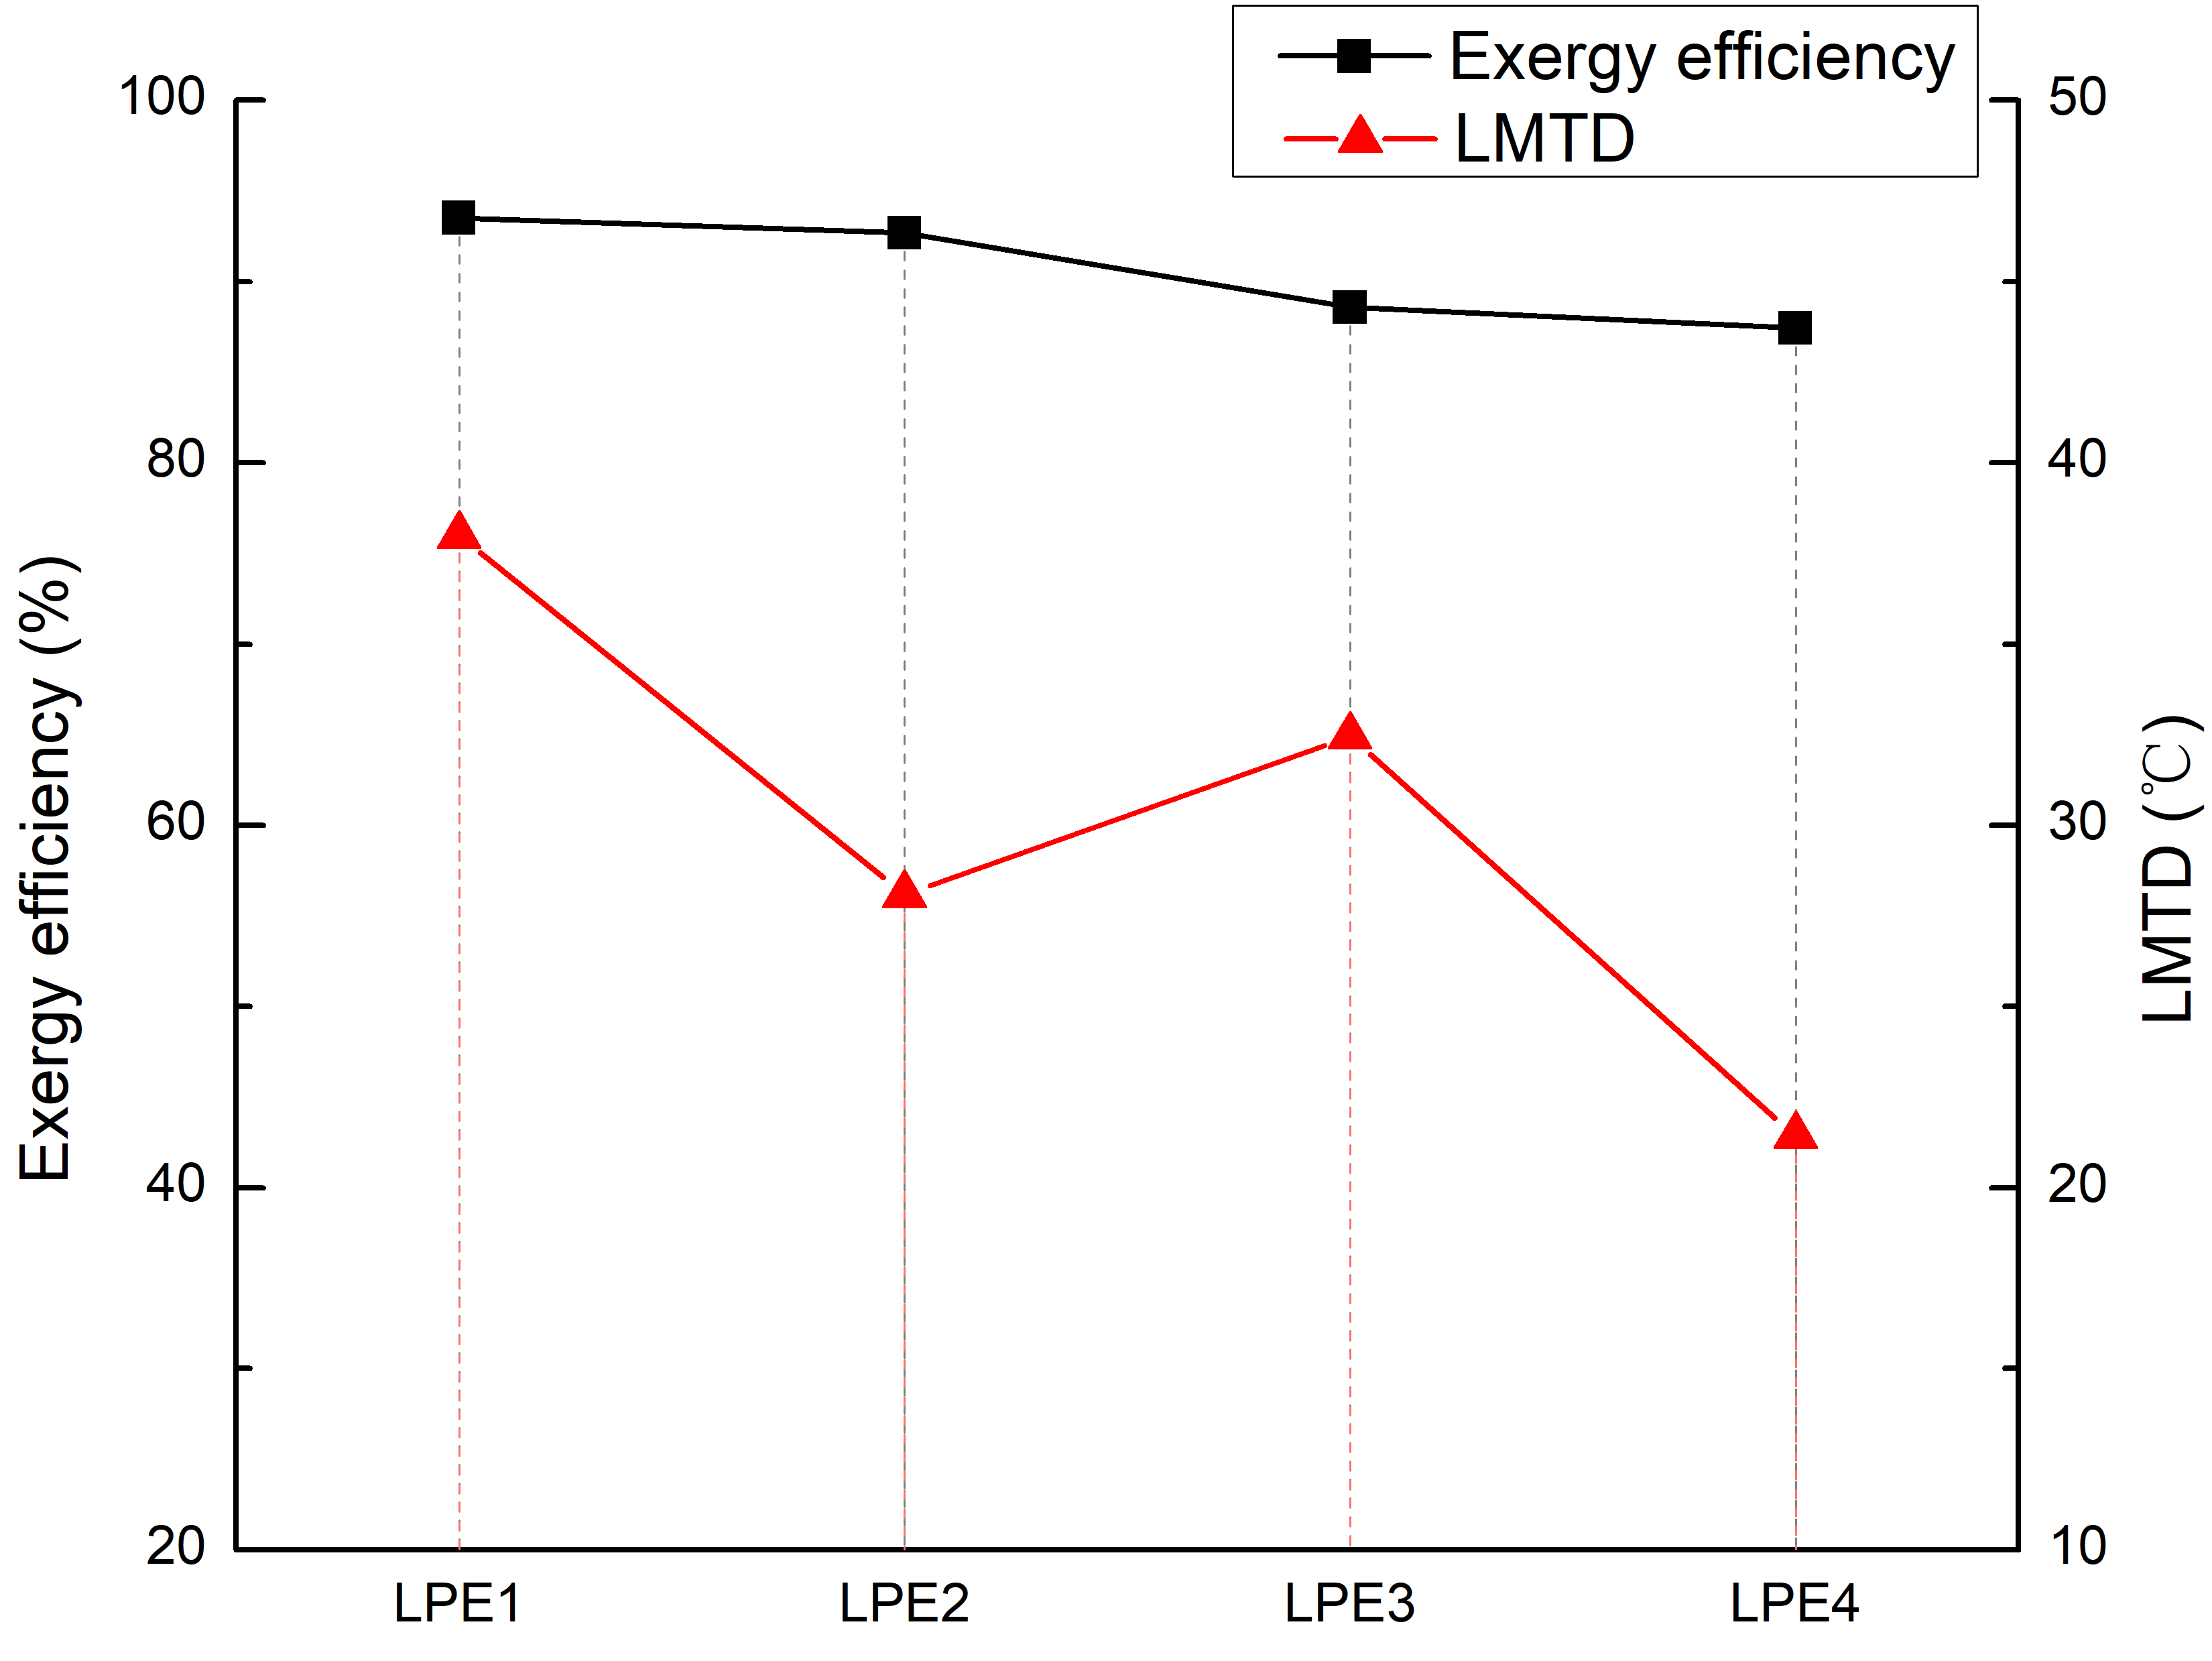
\includegraphics[width=0.6\textwidth]{fig/LPE_exergy_LMTD.png}
\caption{Exergy efficiency and LMTD of LPEs} 
\label{fig:LPE_exergy_LMDT}
\end{figure}


\subsection{Thermodynamic comparison under off-design conditions}
\label{ssub:offdesing_compare}
Given large USC power plants' operation under partial load conditions, it is necessary to study the thermal performance of double-reheat USC power plants under off-design conditions.
Four typical operation conditions--THA load, 75\% THA load, 50\% THA load, and 40\% THA load--were chosen for thermodynamic analysis. 
Fig.~\ref{fig:partload_efficiency} shows the novel and reference systems' exergy efficiency under different load conditions. The exergy efficiencies of both systems decrease as the load decreases.
The exergy efficiencies of the systems are 47.52\% and 46.51\% under the THA load condition. Compared with the reference system, the novel system's exergy efficiency has the increment of 1.01 percentage points and reduces SCE consumption by 5.5\,g/kWh. %What does "has the increment of 1.01" mean?
Under the 75\% THA load condition, the optimized system %The exergy destruction rate of the optimized system?
is 46.56\% and the reference system is 45.90\%, and exergy efficiency decreases to 0.66\%. 
When the load is equal to 50\% THA, the efficiency difference is 0.43\%.
This implies that the novel system can increase exergy efficiency under partial load, but it has more advantages for double-reheat power plants with base loads.

\begin{figure}[htbp]
\centering
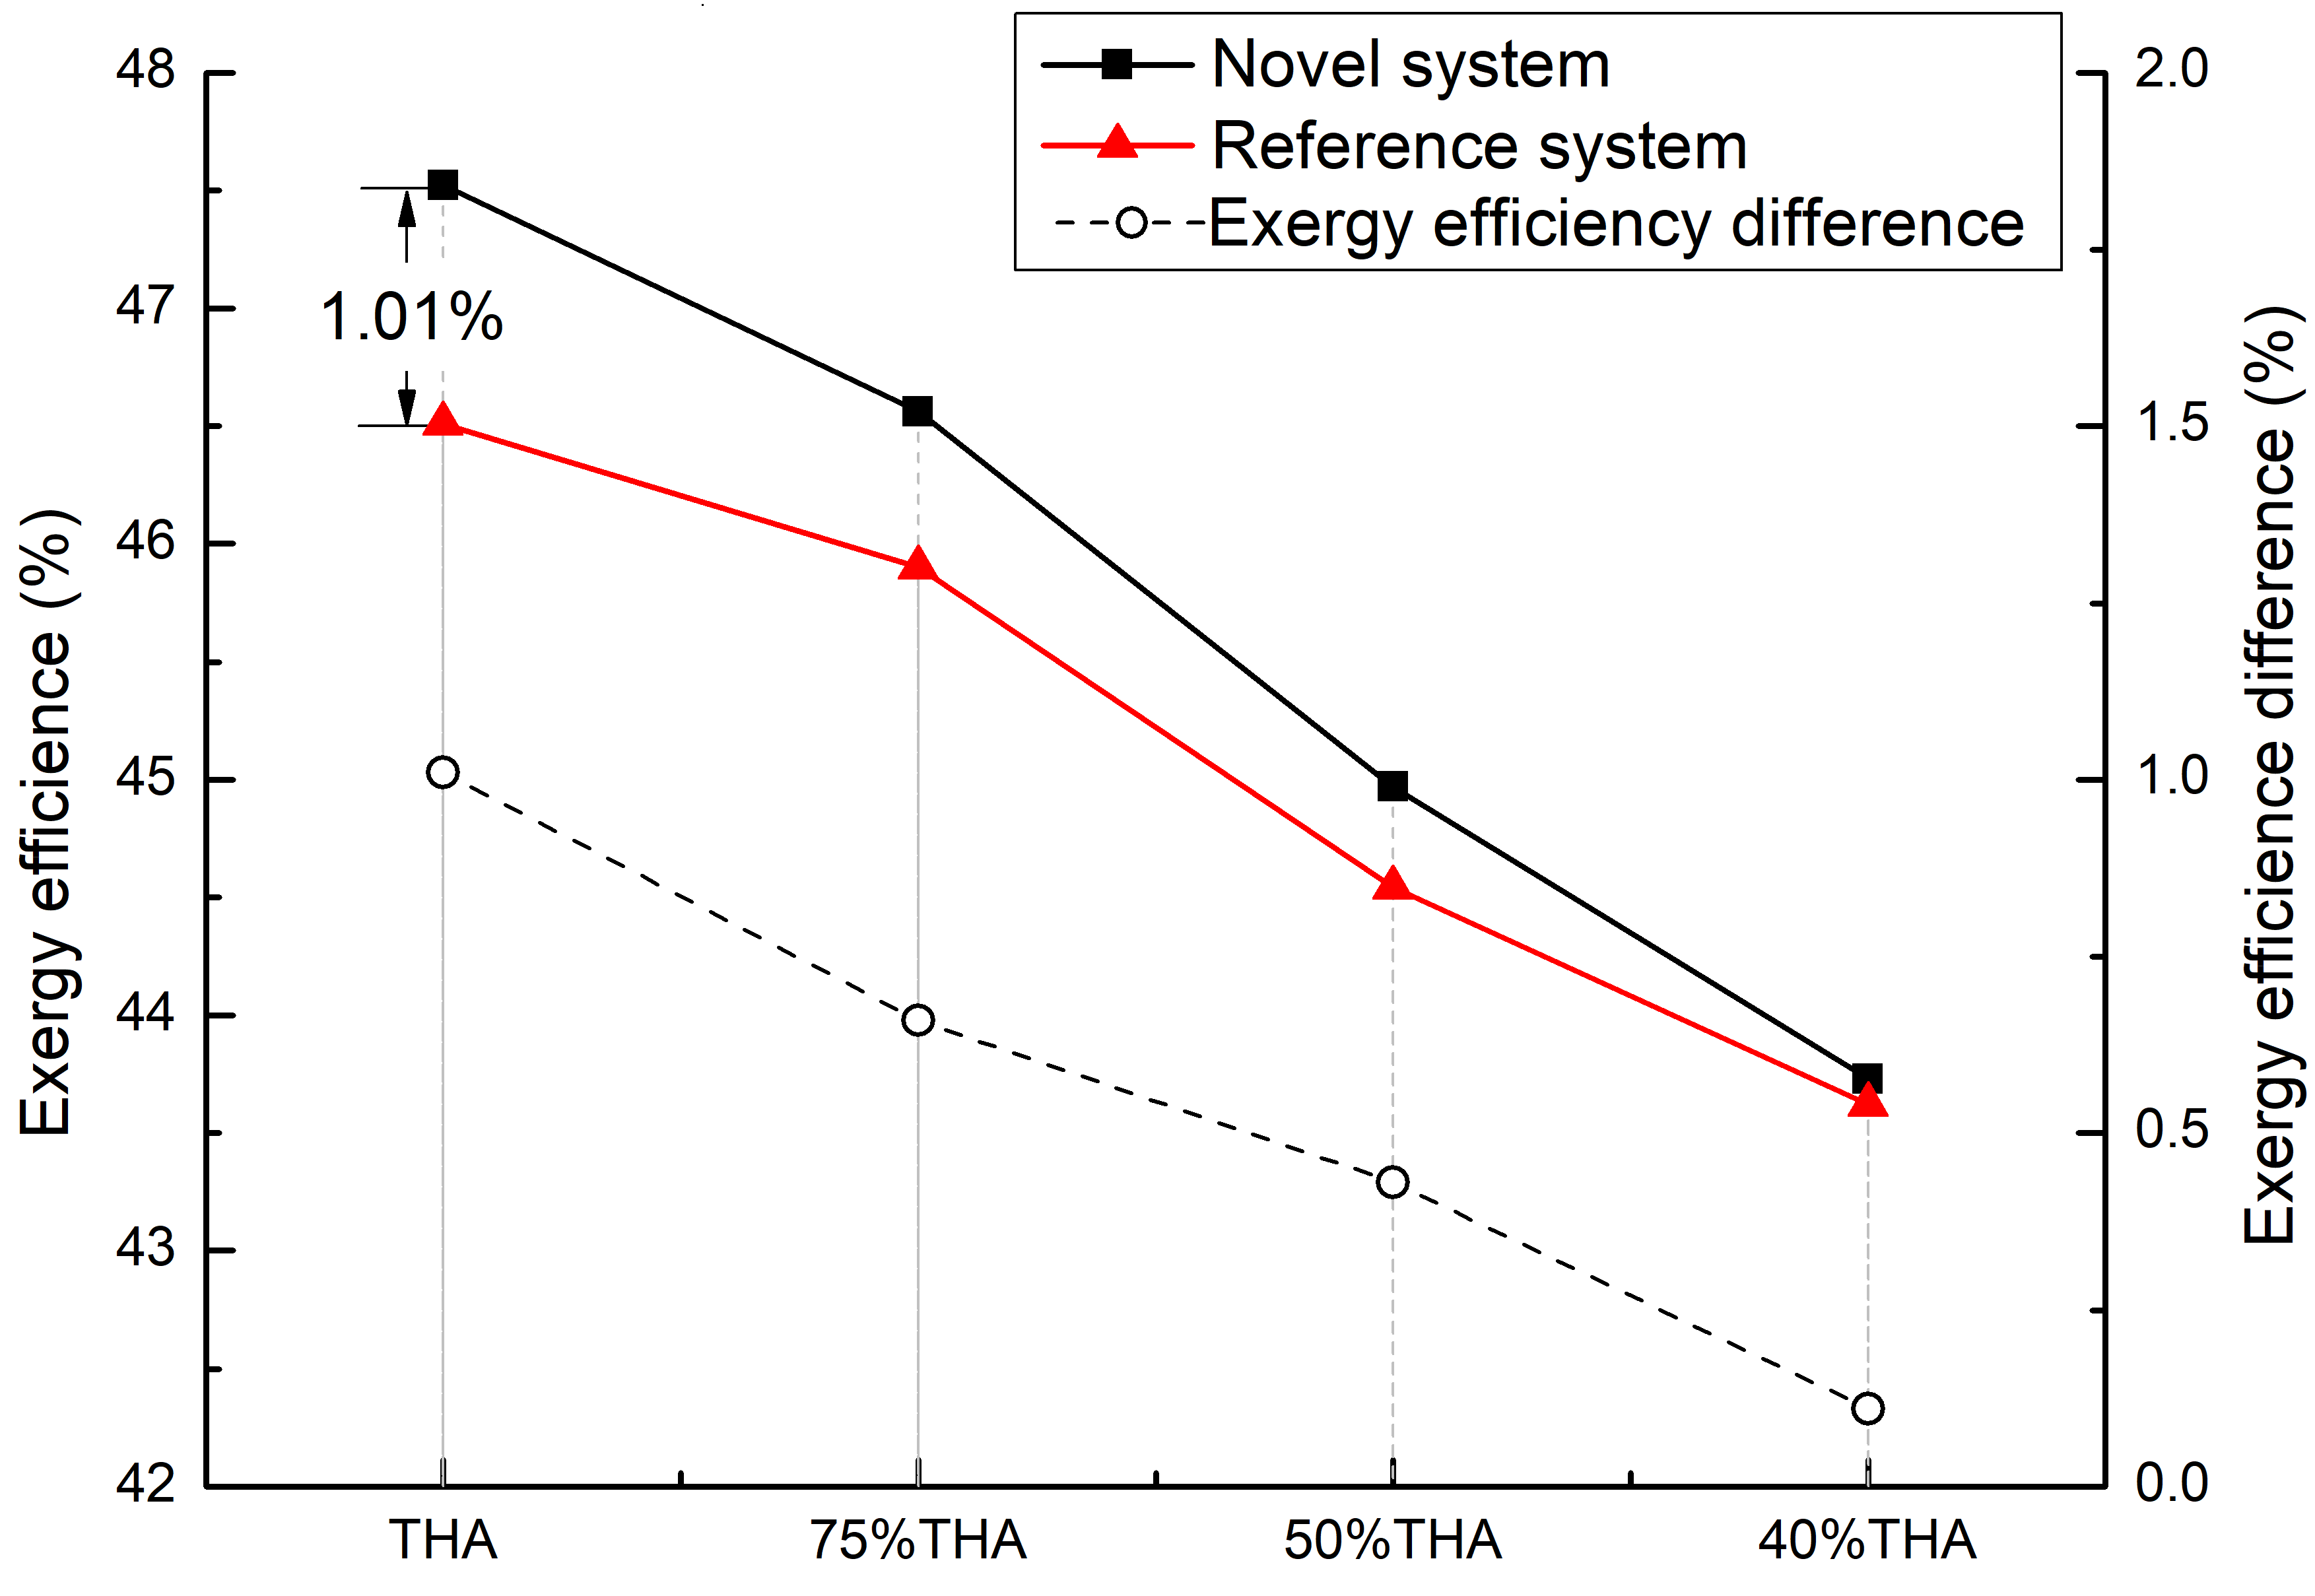
\includegraphics[width=0.6\textwidth]{fig/partload_efficiency.png}
\caption{Exergy efficiency comparison under off-design conditions} 
\label{fig:partload_efficiency}
\end{figure}
  The exergy destruction ratio ($y_{D}$) is used to measure the exergy destruction of a 1\,MW power generation of a unit by a subsystem. It is calculated as follows:
\begin{equation}
y_{D}=\frac{\dot{I}}{P}
\end{equation}

% 用损率差大表明该子系统的节能效果更显著,同时对整个系统的节能效果贡献更大。
% 由图10可以得到新系统引起节能效果从大到小依次为:锅炉、空预系统、回热系统和汽轮机。
% 当负荷从THA逐渐降低可以看到,降负荷对锅炉影响最大,而负荷变化对汽轮机系统影响接近于零。
% 负荷降低到40%,四个子系统优化效果虽然降低但累计值依然优于参考系统,但由于符合降低引起的oher系统用损失的升高导致优化系统相对与参考系统效率增加为0.01%,几乎没有优化效果
% 同时需要指出,由于锅炉本身的用损失很大,所以变负荷对锅炉本身用效率影响很小,而对空预子系统的影响较大。
A large exergy destruction ratio value indicates that the subsystem has more significant energy-saving effects and contributes more to the exergy-saving effects of the entire system.
Fig.~\ref{fig:partload_subsys_exergyrate} shows the exergy destruction ratio difference ($y_{D,reference}-y_{D,novel}$) between the reference system and the novel system.
This indicates that the contribution to energy-saving effects decreases as follows: the boiler, the air preheat subsystem, the regenerative subsystem, and the steam turbine.
As the load decreases from the THA load condition, it can be seen that the load change has the greatest effect on the boiler, while the change in the load condition barely affects the steam turbine.
When the load is reduced to 40\%THA, the four subsystems of the novel system still have lower exergy destruction rates than those of the reference system.
However, the calculated values of these subsystem decrease, 
%Do the edits to the above sentence look right to you?
and the exergy destruction rate increase among the other uncalculated components causes the novel system's exergy-saving effects to decrease.
According to the data presented in Table~\ref{table:system exergy campare}, given the great exergy destruction of the boiler, the decrease in load has little effect on the boiler's exergy efficiency. The air preheat subsystem experiences the greatest effect.


\begin{figure}[htbp]
\centering
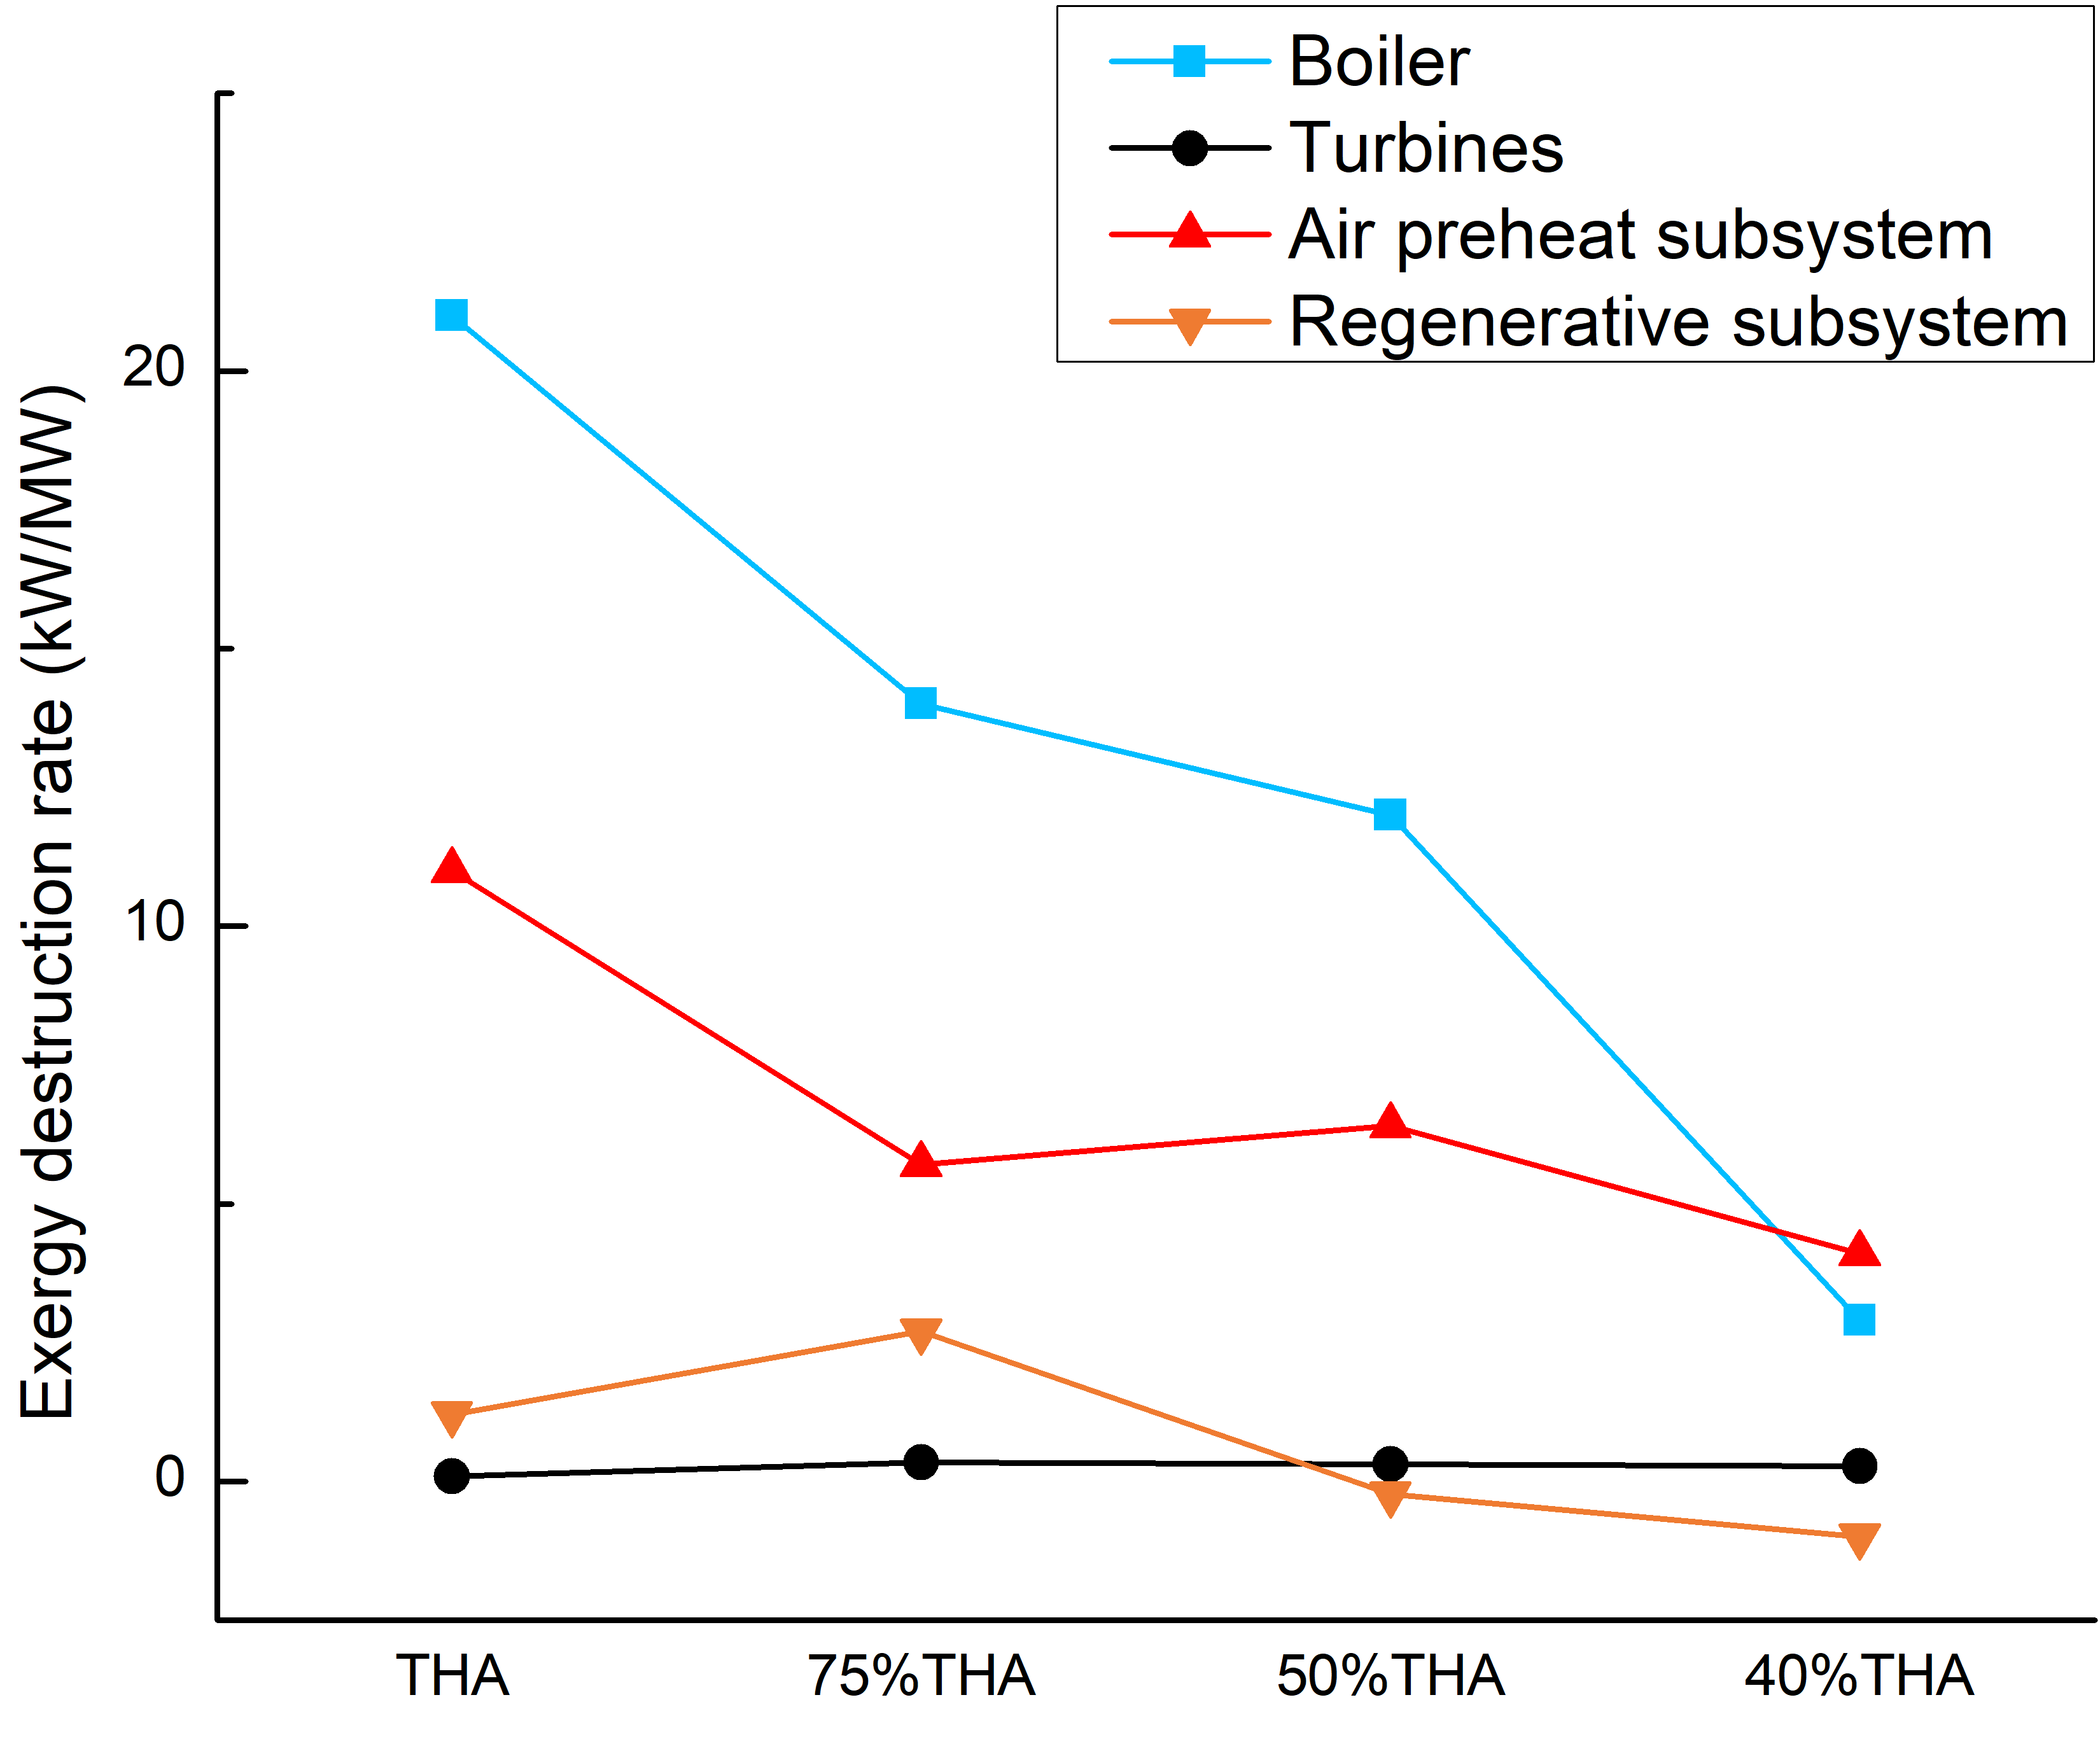
\includegraphics[width=0.6\textwidth]{fig/partload_subsys_exergyrate.png}
\caption{Difference in subsystems' exergy destruction rates under off-design conditions} 
\label{fig:partload_subsys_exergyrate}
\end{figure}

% subsubsection subsubsection_name (end)

\section{Conclusion}
%文章干了什么
This paper proposed a novel system for a 1000\,MW double-reheat ultra-supercritical unit that uses turbine extractions to preheat air and low-pressure economizers to replace the air preheater originally installed in vertical shaft.
Thermodynamic analysis was conducted to reveal the energy-saving effects and thermal performance changes of key components. 
The novel system was found to be effective in overcoming the imperfections
%"overcoming the reference system's imperfections"? 
and may prove an effective method for the optimization of the double-reheat USC unit.
The following conclusions can be drawn from this study: 
 \begin{enumerate}[(1)]
 \item The novel system can improve power generation efficiency up to 48.73\%, which is 1.04 percent higher than that of the reference system under the design condition. The exergy efficiency of the novel system is 47.52\%, which is 1.01 percent higher than that of the reference system.
 \item Thermodynamic analysis indicates that the novel system leads to a decrease in the temperature difference of the air/flue-gas heat transfer process, leading to the cascaded utilization of energy and great reductions in the superheat degree of the third and fifth.
 %"third and fifth extractions"?
\item The novel system changes the mass flow rates of the distribution of extractions, which causes an increment of output power of the generator by 12.09 MW. %I'm not sure what this sentence means. What does it mean to "cause an increment of output power"? Is output power increasing? 
\item The novel system improves the temperature of the secondary air, which improves the fire condition in the combustion chamber.
 The temperature of the secondary air of the reference system under full load is 365$^\circ$C, which is 34$^\circ$C higher than that of the reference system.
\item The novel system theoretically yields remarkable energy-saving effects even under off-design conditions. The simulation results show that the optimized system can reduce SCE consumption by 5.49 g/kWh under the design condition and can even lead to a reduction of 2.9 g/kWh under 50\% THA load.
\end{enumerate}
\section*{Acknowledgments}
This study was supported by the National Basic Research Program of China (Grant No. 2015CB251504).
\section*{References}
\bibliographystyle{elsarticle-num}

\bibliography{bib/reference.bib}


\nomenclature[M]{$\dot{I}$}{exergy destruction rate (MW)}%
\nomenclature[M]{$\dot{Ex}$}{exergy rate (MW)}%
\nomenclature[M]{$\dot{W}$}{work rate or power done by the system (MW)}%
\nomenclature[M]{$\eta_{\uppercase\expandafter{\romannumeral2}}$}{exergy efficiency}%y D
\nomenclature[M]{$y_{D}$}{exergy destruction ratio (MW/MW)}

\nomenclature[M]{$ex$}{specific exergy (MJ/kg)}%

\nomenclature[M]{$h$}{specific enthalpy (MJ/kg)}%
\nomenclature[M]{$s$}{specific entropy (MJ/kg\,K)}%
\nomenclature[M]{$T$}{temperature (K)}%
\nomenclature[M]{$\dot{m}$}{mass flow rate (kg/s)}%

\nomenclature[S]{$in$}{inlet component or system}%
\nomenclature[S]{$out$}{outlet component or system}%




\nomenclature{THA}{turbine heat acceptance}

\nomenclature{AOC}{additional outer steam cooler}
\nomenclature{SCE}{standard coal equivalent}
\nomenclature{USC}{ultra-supercritical}
\nomenclature{LPE}{low pressure economizer}
\nomenclature{EAPH}{turbine-extraction-heated air preheater}
\nomenclature{APH}{air preheater}

\nomenclature{VHP}{super high pressure cylinder}
\nomenclature{HP}{high pressure cylinder}
\nomenclature{IP}{intermediate pressure cylinder}
\nomenclature{LP}{low pressure cylinder}
\nomenclature{ECO}{ economizer}

\nomenclature{RH}{regenerative heater}
\nomenclature{HRH}{high pressure regenerative heater}
\nomenclature{LRH}{low pressure regenerative heater}
\nomenclature{DEA}{deaerator}



\nomenclature{LMTD}{logarithm mean temperature difference} 
\nomenclature{LHV}{lower heating value of fuel} 

\nomenclature{C, H, O, N}{mass fraction of carbon, hydrogen, oxygen, nitrogen of coal} 

\end{document}

\endinput
\%\%
\%\% End of file `article.tex'.
